\expandafter\def\csname CTEX@spaceChar\endcsname{\hspace{1em}}
\documentclass[twoside,AutoFakeBold=true]{ZJUthesis}
\usepackage{diagbox}

% TODO OR NOT TODO: CNN theory fp&bp / TL theory / 

% 该文档中首字符为“%”的均为注释行,不会在论文中出现

% 由于fontsepc包有更新,可能造成在编译过程中的问题
% 如果使用ZJUthesis有问题,可尝试使用ZJUthesisv2
% 如果仍有问题,可换回ZJUthesis,尝试将下面的一行拷至本文档\documentclass之前
% \expandafter\def\csname CTEX@spaceChar\endcsname{\hspace{1em}}

% 论文默认为单面模式,需双面模式请将第一行换为如下所示:
% \documentclass[twoside]{ZJUthesis}
% AutoFakeBold=true 是为解决在Windows系统下,使用xelatex时中文字体不能加粗的问题

% 取消目录中链接的颜色,方便打印
% 如需颜色,请将“false”改为“true”
\hypersetup{colorlinks=false}

%\usepackage[sectionbib]{chapterbib}

\begin{document}
%%%%%%%%%%%%%%%%%%%%%%%%%%%%%
%% 正文字体设定
%%%%%%%%%%%%%%%%%%%%%%%%%%%%%
\fangsong

%%%%%%%%%%%%%%%%%%%%%%%%%%%%%
%% 论文封面部分
%%%%%%%%%%%%%%%%%%%%%%%%%%%%%
% 中文封面内容

% 中图分类号
\classification{TP249}

% 单位代码
\serialnumber{10335}

% 密级,如需密级则将其前“%”去掉
\SecretLevel{无}

% 学号
\PersonalID{21625004}

\title{基于深度学习目标检测的}
% 如果标题一行写不下,就写成两行,在下面的命令里写第二行,不需要两行则注释掉
\titletl{机械臂分拣系统研发}
%\titletl{test}

%英文题目
\Etitle{Development of Robotic Arm Sorting System }
% 如果一行写不下,同中文题目设定,一行写不下则写两行,不需要就注释掉
\Etitletl{Based on Deep Learning Object Detection}

% 作者
%\author{朱雨贺}
\author{}

%\degree{硕士}
\degree{}

% 导师
% \supervisor{陈子辰教授}
\supervisor{}

% 合作导师,如果有的话,去掉注释,
% \cpsupervisor{傅建中教授、姚鑫骅副教授}
\cpsupervisor{}

% 专业名称
% \major{机械制造及其自动化}
\major{}

% 研究方向
% \researchdm{智能制造技术及装备}
\researchdm{}

% 所属学院 
\institute{机械工程学院}

%论文提交日期
\submitdate{2019年1月25日}

% 答辨日期
\defenddate{2019年3月15日}
\defenddateE{March 15th, 2019}

% 生成封面
\makeCoverPage

%%%%%%%%%%%%%%%%%%%%%%%%%%%%%%
%% 中文题名页内容
%%%%%%%%%%%%%%%%%%%%%%%%%%%%%%
% 论文评阅人信息 注意两字名与三字名,两字职称与三字职称的写法,便于对齐
% 多余的名额直接注释掉即可,比如三个评阅人,把评阅人D,E注释掉即可
\reviewersA{\hspace{1.5em}\hspace{1.5em}\hspace{1em}}
\reviewersB{\quad \hspace{1.5em}\hspace{1.5em}\hspace{1em}}
\reviewersC{\hspace{1.5em}\hspace{1.5em}}
\reviewersD{\hspace{1.5em}\hspace{1.5em}\hspace{1em}}
\reviewersE{\hspace{1.5em}\hspace{1.5em}\hspace{1em}}

% 答辩委员会信息,如果某一个单位比较长, 
% 请在其它较短后面补上{hspace{Xem}},X是比最长的单位名少几个字
% 如果实际人数少于6人,多余的注释掉即可
\chairman{\hspace{1.5em}\hspace{1.5em}}
\commissionerA{\quad \hspace{1.5em}\hspace{1.5em}\hspace{1em}}
\commissionerB{\quad \hspace{1.5em}\hspace{1.5em}}
\commissionerC{\quad \quad \quad }
\commissionerD{\quad \hspace{1.5em}\hspace{1.5em}\hspace{1em}}
\commissionerE{\quad \hspace{1.5em}\hspace{1.5em}}

% 生成中文题名页
\maketitle
 
%%%%%%%%%%%%%%%%%%%%%%%%%%%%%%
%% 原创声明与版权协议页
%%%%%%%%%%%%%%%%%%%%%%%%%%%%%%

\SignautreDateA{}{}{}
\SignautreDateB{}{}{}
\SignautreDateC{}{}{}
% 生成原创声明与版权协议页
\makeOSandCPRTpage

%%%%%%%%%%%%%%%%%%%%%%%%%%%%%%
%% 论文部分开始
%%%%%%%%%%%%%%%%%%%%%%%%%%%%%%
\ZJUfrontmatter

%%%%%%%%%%%%%%%%%%%%%%%%%%%%%%
%% 致谢页
%%%%%%%%%%%%%%%%%%%%%%%%%%%%%%
% \begin{thanks}
两年半的求学生涯,在各位老师和朋友的帮助和支持下,即将画上一个圆满的句号。
回顾过往,虽然辛苦却也收获良多,转眼已到毕业的时候,心中难免不舍。
在此,我要向所有支持我的人表达衷心的谢意。

首先,我要感谢我的导师陈子辰教授对我的培养。
陈老师渊博的知识、认真的科研精神、诲人不倦的高尚品德以及谦和的人格魅力对我产生了深远的影响。
陈老师虽然忙身于教学与科研重任,但仍然经常指导我,特别注重我们独立思考能力能力以及工程实践能力的培养。
此外,陈老师还关心我们的生活,注重我们人格的培养。
有幸能成为陈老师的学生,我不仅学会了如何科研,更学会了如何做人。

我还要特别感谢傅建中教授。
傅老师在我的整个硕士生涯中,对我的科研生活起到了极大的知道作用。
傅老师身为实验室的带头人,为实验室的师生营造了一个自由向上,积极进取的科研氛围。
在傅老师的带领下,实验室科研成果不断。
也得益于实验室自由的环境,在科研之外,各个同学在各个领域都有所建树,全面发展。
同时,傅老师在我的毕业设计中,细心指导了我的毕设选题、创新点发掘、论文撰写,
使我能够顺利完成毕业论文的撰写。生活中,傅老师平易近人,亦师亦友。

我还要特别感谢姚鑫骅副教授。
姚老师在我的硕士生涯中影响巨大。姚老师在我的日常课业、科研项目以及挑战杯项目中起到了很大了指导作用。
姚老师具有渊博的知识、严谨的治学态度,是我在科研项目中的带头人。
同时,姚老师不仅在科研中给予了我莫大的帮助,在生活以及心理方面,姚老师也不断地鼓励着我。
帮助我顺利完成了硕士学业。

感谢沈洪垚副教授、贺永教授、吴森洋老师、郑亚平老师、周芳丽老师,
在课题组进行科研的过程中,他们在很多方面都影响和帮助着我。

同时,我还要感谢所有教导、帮助、关心过我的老师。在整个本科和硕士学习生涯中,
他们给予了我莫大的帮助,他们的帮助也让我成长了许多。

感谢实验室已经毕业的王博、延健磊、代晓萌、饶成晨、兰刘健、刁怀东等师兄师姐在科研、求职
以及生活中对我的帮助。感谢实验室的林志伟、栾丛丛、孙扬帆、牛小淼、张德明、刘加朋、张承谦、
谢明君、孙元等博士生给予我的帮助。感谢与我同一届的孙伟俊、刘森鑫、黎清雨、干胜、赵耀、刘丞哲、
夏能、王鹏、严梦玲、黄天玺、周瑞剑等同学,我们共同求学于同一个实验室,互相帮助,共同克服科研路上
的难题。感谢史璇珂、吕健冉、杜旺哲、王润秋、刘诗怡、刘冰、林炜奕、方泽华、叶潇翔、田佳陇、李霄铿等
师弟师妹,在给予我帮助的同时,也为实验室带来了新的活力。

感谢女朋友申佳佳的帮助、包容与鼓励,我们一起求学、求职,她在我低谷时给予我温暖的鼓励,在我迷茫时
为我出谋划策,是她让我更加自信、更加坚定自己的方向。

感谢同寝室的武欣、黎清雨、苟华伟同学,感谢他们在生活上给予我的帮助和支持。

最后,我要感谢的是我的家人,感谢他们这么多年来对我的养育和培养。
二十年寒窗苦读,是他们的支持和鼓励让我走到了今天。
他们默默付出,不图回报,他们的爱是我最宝贵的财富。

如今,我即将离开学校,步入下一段新的旅程,衷心感谢这些年来所有帮助过我的人,谢谢!

% \hfill xxx 该命令为右对齐
\hfill 朱雨贺

\hfill 2019年1月于求是园

\end{thanks}


%%%%%%%%%%%%%%%%%%%%%%%%%%%%%%
%% 摘要
%%%%%%%%%%%%%%%%%%%%%%%%%%%%%%
\begin{abstract}
待填

\keywords{深度学习,目标检测,分拣系统,机械臂,云平台}
\end{abstract}


%%%%%%%%%%%%%%%%%%%%%%%%%%%%%%
%% 英文摘要
%%%%%%%%%%%%%%%%%%%%%%%%%%%%%%
\begin{englishabstract}
Sorting operation is a very common scenario in the manufacturing industry. Due to its repetitive nature, sorting operation
has become one of the important application scenarios of industrial robots. Conventional automatic sorting systems use traditional
image methods which manually struct features for specific workpiece and use templates to match workpiece positions and then classify them.
This method has low accuracy, poor robustness and weak portability. At the same time, the lack of image talents among domestic manufacturing practitioners has
raised the threshold for the application of vision-based automatic sorting in manufacturing. Therefore, for the algorithmic effect of the 
vision-based automatic sorting system and its application threshold, this paper designs and implements an automatic sorting system based on 
deep learning and a cloud platform for object detection algorithm training of the automatic sorting system.

Firstly, based on the situation of large amount of deep learning and the specific scene of the automatic sorting system, the overall architecture
of the automatic sorting system based on deep learning is designed, and the performance level of the automatic sorting system (grab the workpiece and 
acquire the image), The control plane (image processing and robotic arm control) and the background level (target detection algorithm training and selection) 
are organically separated, so that the modules of the automatic sorting system exhibit a loosely coupled relationship, 
facilitating the development of subsequent deep learning cloud platforms. At the same time, combined with the automatic sorting system using the depth detection-based
 target detection algorithm, the hardware selection, model selection and communication mode selection are targeted. 
 For the camera and the robot arm, the design and implementation of the hand-eye calibration and the manipulator control instruction scheme were carried out.

Secondly, the image processing module of the automatic sorting system is designed. 
The traditional image processing algorithm and the deep learning target detection algorithm are organically combined to reduce the 
use delay of the image processing module of the automatic sorting system. 
At the same time, because the training of deep learning model requires a large number of data sets, 
combined with the fact that the amount of data in the manufacturing factory is small, and the data is time-consuming and labor-intensive, 
the migration learning technology is used to improve the performance of the training model under a small number of labeled data sets. 
Then combined with the actual hardware configuration of the automatic sorting system, 
select YOLOv3-tiny as the target detection algorithm model configuration of the automatic sorting system.

Thirdly, a cloud platform for training deep learning target detection algorithms is designed and implemented. 
Combined with the actual use scenarios and user requirements of the cloud platform, a Web-server development solution was designed. 
Completed the development of web front-end pages and server-resident programs. 
The user can obtain a customized deep learning target detection model through a simple web page operation.

Finally, for the image processing module of the automatic sorting system, 
the design experiment verifies the superiority of the configuration selection of the target detection model, 
and collects the success rate of the automatic sorting system for the workpiece and the success rate of sorting, 
and verifies the automatic sorting system. Practicality and stability. The performance of the web front-end page and the server 
background of the deep learning cloud platform was tested. The experimental results prove that the deep learning cloud platform has good stability.

The deep learning-based automatic sorting system designed in this paper not only improves the target detection algorithm of the traditional automatic 
sorting system, but also optimizes the hardware selection and model training, and proposes the deep learning cloud platform. 
The application threshold of the system in the manufacturing industry is greatly reduced.

\TeX\index{\TeX}

\englishkeywords{Deep Learning, Object Detection, Sorting System, Cloud Platform, Robotic Arm}

\end{englishabstract}


%%%%%%%%%%%%%%%%%%%%%%%%%%%%%%
%% 插图列表
%%%%%%%%%%%%%%%%%%%%%%%%%%%%%%
%\ZJUListofFigures

%%%%%%%%%%%%%%%%%%%%%%%%%%%%%%
%% 表格列表
%%%%%%%%%%%%%%%%%%%%%%%%%%%%%%
%\ZJUListofTables

%%%%%%%%%%%%%%%%%%%%%%%%%%%%%%
%% 目录页
%%%%%%%%%%%%%%%%%%%%%%%%%%%%%%
\ZJUcontents 

%%%%%%%%%%%%%%%%%%%%%%%%%%%%%%
%% 正文内容部分开始
%%%%%%%%%%%%%%%%%%%%%%%%%%%%%%
\ZJUmainmatter

%%%%%%%%%%%%%%%%%%%%%%%%%%%%%%%
%%% 第一章 绪论
%%%%%%%%%%%%%%%%%%%%%%%%%%%%%%%
\chapter{绪论}

%%% 1.1 论文研究背景及意义
%%%%%%%%%%%%%%%%%%%%%%%%%%%%%%% 
\section{论文研究背景及意义}
\subsection{研究背景}

人工智能的迅速发展将深刻改变人类社会生活,改变世界。为此,国务院在2017年7月8日向
各省、自治区、直辖市人民政府等印发了《新一代人工智能发展规划》     \cite{GWY:2017}。
此规划是为了推动人工智能
快速发展,造福民生。其中,“人工智能+”是其中的重要环节。所谓“人工智能+”,就是将人工智能与各个传统行业深度融合,
深入改造各个传统行业,帮助传统行业转型,创造新的产业形态。而智能制造则是人工智能与制造业的深度融合。十八大以来,
“制造业转型升级”等战略被逐步提出,但对于中国制造来说,要实现转型升级,首先要考虑由劳动密集型向技术密集型转变。而
人工智能技术与制造业的融合可以代替大量劳动力,实现工业自动化,助力“中国制造2025”,帮助中国制造转型升级。

工业机器人,按照ISO 8373    \cite{ISO:1994}
的定义,是面向工业领域的多关节机械手或多自由度的机器人。工业机器人通过预先编写
的程序可以实现重复性动作,以此可来代替一些重复性的人工工作,是制造业中非常重要的劳动力代替工具。根据国际机器人联合会发布的
2012年世界机器人研究报告,在2011年年底,世界上运行中的工业机器人数量达1153000。可以说,工业机器人的每次技术进步,都能带来
制造业工作效率质的提升。

分拣作业是制造业中非常常见的一种作业场景,由于其重复性强、作业场景单一的任务特性,分拣作业成为工业机器人的重要应用场景之一。
传统的工业分拣采用人工方法,不但耗时耗力,而且无法满足自动化长时间作业,影响生产效率的提升。而传统的工业机器人自动分拣系统,
采用预先编程的工业机器人进行工业分拣,虽然能够实现重复性动作的复现,但由于工业机器人无法根据实际情况改变自身动作,所以这种系统
对分拣件的摆放位置有严格的设定,且该系统只能进行分拣,无法进行分类。因此,近年来,越来越多的学者将机器视觉应用到工业机器人当中,
使机器人具备人眼功能,能够根据工件位置自适应地调整机器人动作,并且能够实现分拣和分类。基于机器视觉的工业机器人系统具备更好的鲁棒性,
因此越来越多的机器视觉工业机器人投入到实际应用中,不仅提高了生产产品质量,更保证了工业化生产的效率  \cite{CJF:2011}。

机器视觉技术是利用机器代替人眼做各种测量和判断的技术    \cite{BZG:2015}。
工业自动分拣系统主要由机器人、视觉传感装置、
图像采集装置和图像处理系统构成  \cite{ZWH:2018},
其中机器人模块主要执行图像处理系统所返回的指令,其他模块构成了机器视觉模块,
负责获取所需识别物体的位置及类别。由于机器人模块受环境影响较小,而图像处理模块需要满足工业环境中的实时性和快速性要求,而且需要对
工厂复杂多变的环境有较高的适应性。因此,机器视觉中的目标检测算法是整个视觉自动分拣系统中的核心。

人工智能的高速发展必定伴随着对各行各业的改造。以深度学习为代表的算法也在不断颠覆各种传统机器视觉算法。将深度学习应用到基于视觉的工业分拣
系统中,不仅能够提高视觉识别的效果,而且得益于深度学习的端到端的特性,系统的可移植性也可以得到提高。本文研发的基于深度学习的机械臂分拣系统
及其云平台,将深度学习应用到自动分拣系统的核心模块:目标检测,并且研发出一套基于深度学习,用于训练目标检测算法的云平台,降低视觉应用门槛,
具备更强的通用性。

\subsection{研究意义}

随着“中国制造2025”的提出,中国正迈向“制造大国”到“制造强国”的道路。中国制造业自动化转型迫在眉睫。工业机器人,作为
制造业中不可或缺的生产工具,在制造业自动化中扮演着重要角色。工业机器人任何技术上的提升必定带来制造业生产效率的提升。
因此,对工业机器人的技术研究对实现“中国制造2025”具有重要意义。

作为工业机器人应用的重点和难点,工业分拣系统具备大多数工业机器人应用的技术应用场景。工业自动分拣系统的研究突破势必带动工业机器人
技术的进步。工业自动分拣系统主要包括图像采集模块、图像处理模块、机器人模块。其中,图像采集模块主要用于获取分拣件图像信息,作为图像处理
模块的输入;图像处理模块主要根据图像采集模块采集得到的图像信息,进行计算,得到分拣件位置和类别信息,并将该信息发送给机器人模块执行;机器人模块
根据分拣件位置和类别信息,对分拣件进行抓取并放到合适位置。这其中,图像处理模块是整个系统的中枢,决定了整个系统的实时性和准确性。一个好的图像
处理模块带来的系统性能提升是其他模块无法带来的。

分拣系统中用到的图像处理算法主要为目标检测算法。目标检测算法可以根据是否应用深度学习技术,将之分为传统目标检测算法和基于深度学习的目标检测算法。
传统的目标检测算法需要人为构造特征,且针对不同检测物体需要构造相应的特征。当需要检测的物体数量变多并且经常发生变化时,传统的目标检测方法就会显得
捉襟见肘。而基于深度学习的目标检测算法可以实现端到端的训练和预测。同时,深度学习端到端的特性既方便了模型的训练,又方便模型的移植。针对不同的检测
场景,只需要标注相应数量的数据,利用迁移学习    \cite{TransferL:2010}
技术,在ImageNet  \cite{ImageNet:2009}
的预训练参数上进行fine-tune,即可得到良好的可用模型。

鉴于以上特性,根据当前工业自动分拣系统及我国制造业特性,提出了本论文的基本设想,即开发一套基于深度学习的机械臂分拣系统,同时将深度学习模型的训练过程
开放到云平台。本论文的设想分两部分:一是将基于深度学习的目标检测算法应用到工业分拣系统当中,验证其可行性及效果;二是开发基于深度学习的目标检测模型训练
云平台,帮助制造业从业者生成他们所需的目标检测模型。相对应地,本论文有如下两部分意义:一是研究深度学习在工业分拣系统中的应用效果,提高工业自动分拣系统的
分拣质量及鲁棒性;二是从我国制造业从业者深度学习知识普及度不高的事实出发,将深度学习模型的训练过程封装为对制造业从业者友好的网页界面,从而普及深度学习在工业
自动分拣系统甚至是整个制造业中的应用。

%\begin{figure}
%\centering
%\includegraphics{}
%\caption{}
%\label{Figflag} 
%\end{figure}

%%% 1.2 国内外研究现状
%%%%%%%%%%%%%%%%%%%%%%%%%%%%%%
\section{国内外研究现状}
%%% 1.2.1 目标检测算法研究现状
%%%%%%%%%%%%%%%%%%%%%%%%%%%%%%
\subsection{目标检测算法研究现状}
目标检测是机器视觉中的一个重要问题,在轨迹跟踪、自动驾驶、工业分拣等生活及工业领域都具有重要的应用和研究价值。早期的目标检测算法
主要是人工构造特征,通过模板和传统机器学习方法进行检测。然而,2012年,Hinton等人提出了AlexNet   \cite{NIPS2012_4824},
在ImageNet
的表现超出第二名41\%,将深度学习的革命性效果带到大众眼前。深度学习在图像分类任务上的良好表现,促使各界学者纷纷在各自的领域应用深度学习,
由此催生出一批基于深度学习的优秀算法。目标检测任务也不例外。

自目标检测的概念提出以来,国内外学者针对目标检测算法进行了一系列探索。在深度学习兴起之前,传统的目标检测算法大致分为目标实例检测和传统
目标类别检测两类    \cite{MBJC:2018}:
\begin{enumerate}
    \item{目标实例检测,即通过模板和人工提取的特征点,获得模板与检测对象的对应关系,检测出目标对象。}
    \item{目标类别检测则通过使用传统的机器学习方法,根据人工提取的特征和选定的分类器,检测出实现定义好的有限几种类别。}
\end{enumerate}

2004年,Lowe等提出在目标实例检测方面应用极为广泛的SIFT  \cite{Lowe2004}
算法,该算法使用高斯模糊来实现尺度空间,使用高斯差分函数
进行极值检测,再通过对各个因素的判定和筛选,得出匹配度高、抗噪性强的关键点。但该算法存在复杂度高、速度慢、对于特征不明显图像很难提取特征
点等问题。针对这些问题,Ke等人同年提出了PCA-SIFT    \cite{PCA-SIFT:2004}
算法。该算法引入PCA方法对SIFT算法中的向量进行降维,以提高匹配效率。但
由于降维损失了部分信息,因此该算法虽然提高了匹配效率,但匹配效果具有局限性。同样基于SIFT,2006年提出的SURF  \cite{SURF2006}
算法则引入了Hessian
矩阵,减小了计算量,提高了目标检测的速度。而目标类别检测方面,使用较多的则是基于AdaBoost    \cite{AdaBoost1996}
的系列算法。AdaBoost算法是一种Boosting算法,能够将多个弱学习器,通过调整训练集样本权重的方法,组合为一个强学习器。

传统的目标检测算法,其目的都是在人工提取丰富特征点的前提下,尽可能减少计算量,从而提高计算效率,提高识别速度。但人工提取特征虽然易于理解,
简单直观,但无法应对大量类别的识别,在目标识别体发生变化时,需要针对性地再次进行繁杂的特征设计和提取工作。而基于深度学习的目标检测算法,使用神经
网络提取图像底层和高层特征,不仅能够提取出更加丰富、表达性更强的特征,而且不需要人工参与特征的提取,还能做到端到端的训练和预测。

基于深度学习的目标检测算法分为两类。一类是基于分类的目标检测算法(two-stage),另一类则是以回归的方式来进行目标检测的算法(single-stage)。
顾名思义,two-stage的方法,采用两步来进行目标检测:1. 生成可能区域(Region Proposal)并且使用CNN提取特征。2. 使用分类器分类并修正位置。这类方法
的代表是R-CNN   \cite{RCNN:2014}。
2014年,Ross等人提出了R-CNN。该算法使用Selective Search获得候选区域,然后进行归一化,作为CNN网络的输入。再使用神经网络获取候选区域的特征,最后利用
多个SVM分类器进行分类。R-CNN大幅度提高了目标检测的准确率,但由于R-CNN是对所有的候选区域进行特征提取和计算,多个候选区域之间的重叠区域重复计算了多次,导致
了大量重复计算,降低了运算效率,并且由于计算过程复杂,计算过程中需要存储大量中间数据,需要消耗大量的存储资源。因此,R-CNN的实时性不强,并且非常占用存储资源。
针对R-CNN的重复计算性问题,2014年,何凯明等人提出了SPP-Net     \cite{SPP-NET:2014}
。SPP-Net不同于R-CNN对所有候选区域进行特征提取,而是使用CNN对整张图片进行一次特征提取,大大减小了计算量,并且在R-CNN的最后一个CNN层之后,加入了
SPP层。但SPP-Net依然没有解决R-CNN占用过多存储空间的问题。
2015年,Fast R-CNN  \cite{Fast-RCNN:2015}
在SPP-Net的基础上进行了改进,将SPP层进行了简化,将分类和边框回归问题进行了合并,并且引入SVD分解,减小了计算量。Fast R-CNN相对于SPP-Net提高了计算速度,减小
了内存占用,但仍然使用Selective Search的方法选取候选区域,并进行大量计算,其计算速度依然不尽如人意。针对候选区域选择的问题,Faster R-CNN    \cite{Faster-RCNN:2015}
使用RPN网络代替了Selective Search,标志着基于深度学习的目标检测算法走上了真正端到端的计算。但由于Faster R-CNN仍然使用了Fast R-CNN中的ROI层,导致其在小目标的检测任务上
效果不尽如人意。并且由于two-stage本身思路的限制,two-stage系列算法中最快的Faster R-CNN也只能达到5FPS。因此,研究者们提出了另外一种思路:
single-stage。即将目标检测和分类问题直接转化为回归问题,去掉选择候选区域及提取特征这一步,直接通过整图得到检测物位置和类别。这一系列算法的代表是YOLO    \cite{YOLO2016}
算法。YOLO算法将整张图片划分为S×S个网格,各个网格负责检测中心落在该网格内的检测物体,包括检测物位置和类别信息。该算法通过舍弃了一定的精确度换取了速度的大幅度
提升,其检测速度最高可达45FPS。但检测精度比Faster R-CNN要差。同年提出的SSD  \cite{SSD2016}
算法,则结合了YOLO和Faster R-CNN的优点,在保证检测精度的同时,兼顾检测速度。YOLO算法发表的次年,即2017年,YOLO的作者又提出了YOLOv2  \cite{YOLO9000:2017}
算法,该算法通过在卷积层后面加入BN层、加入K-Means聚类方法等方式,同时提高了检测精度和速度。该算法代表了2017年业界最先进的目标检测算法。2018年,YOLOv3   \cite{YOLOv3:2018}
基于YOLOv2做了一些设计细节的改进,在保持高检测速度的前提下,再次提高了检测精度。总之,针对不同的应用场景,two-stage算法和single-stage算法各有其适用范围。没有不好的算法,只有
合适的使用场景。


%%% 1.2.2 分拣系统研究现状
%%%%%%%%%%%%%%%%%%%%%%%%%%%%%%
\subsection{基于视觉的自动分拣系统研究现状}


基于视觉的分拣系统,利用机器视觉技术,对目标进行识别与跟踪,将目标位置和类别信息反馈给机械臂控制模块,从而控制机械臂完成目标工件的分拣工作。基于视觉的分拣系统在
国外的研究已经比较成熟,应用场景正在不断扩大。国内相关研究起步较晚,但近年来也在加大研究力度,逐步缩小与国外的研究差距。

由于自动分拣系统在各个领域应用十分广泛,而不同领域所需使用的算法及机械臂均不相同,因此,在各个领域,均有相应的自动分拣系统研究成果。如水果分拣领域,该文献  \cite{DT:2018}
提出了一种基于视觉的水果自动分拣方案,能够根据分类器分出水果的质量好坏,根据水果横径尺寸讲水果分为大、中、小果,同时能够根据水果表面颜色信息对水果成熟度做出判断。在制药领域,
有文献  \cite{YP2017}
设计出一种药片自动分拣系统,通过药片图像的预处理,进行药片缺陷的检测与分类,并在此基础上实现了药片的自动分拣。制造业领域,自动分拣系统主要用于工件的分拣,并且在分拣过程中可以做到
工件的无损检测。此文献  \cite{GJ2017}
设计了一个工件智能分拣平台,能够对工件进行在线动态分拣,使得分拣效率大幅度提升。

国内的自动分拣系统研究中,对其中的目标检测算法也做了许多创新性的研究。比如,伍锡如等人  \cite{WXR2016}
在进行工件目标检测时,结合了传统图像算法和深度学习算法。在工件定位阶段使用传统图像算法做匹配以确定工件位置,在工件分类时则使用CNN进行分类。
此外,由于我国电子商务告诉发展,国内每年上亿包裹,也催生了快递领域自动分拣系统的应用。如该文    \cite{kuaidi}
中提到的物流分拣机器人,通过视觉技术,可根据商品的重量及发往地等信息进行快速分拣,极大地提高了快递发货周期,提高服务水平。
其中运用到了大量的视觉技术,如数量检测、形状识别等。
%%% 图片组合:subfigure和minipage
\begin{figure}[t]
    \centering
    \subfigure[FANUC M-1iA型号机器人]{
        \label{fig:robot_example:a}
        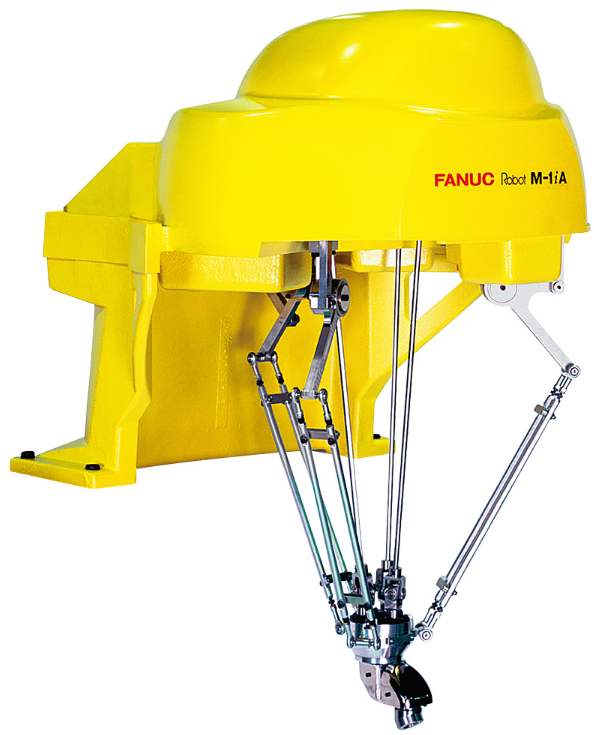
\includegraphics[width=0.25\columnwidth, height=0.2\textwidth]{pic/chap1/FANUC-M-1ia.jpg}
    }
    \subfigure[FlexPicker机器人]{
        \label{fig:robot_example:b}
        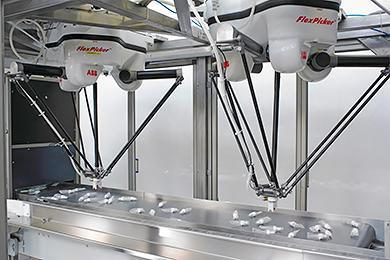
\includegraphics[width=0.25\columnwidth]{pic/chap1/FlexPicker.jpg}
    }
    \subfigure[物流自动分拣机器人]{
        \label{fig:robot_example:c}
        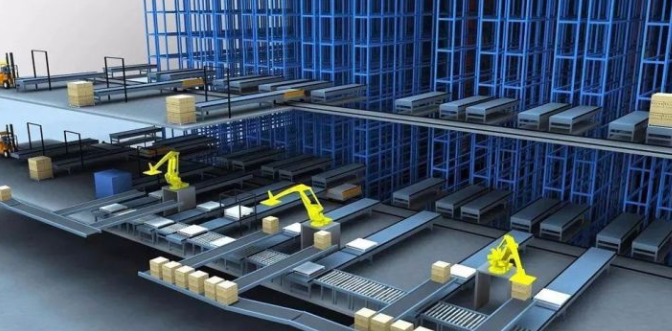
\includegraphics[width=0.5\columnwidth]{pic/chap1/wuliu.jpg}
    }
    \caption{自动分拣机器人实例}
    \label{fig:robot_example}
\end{figure}

目前,国内有多家提供自动分拣解决方案的公司。如深圳辰视智能科技公司,该公司采用传统机器学习方法与深度学习结合的方式定位图像中的目标,引导机械臂对目标采取
相应的操作,以高效低成本的方式为机器人厂家提供机器视觉相关的解决方案。

国外方面,著名的机器人生产厂商如日本的FANUC、EPSON,瑞典的ABB以及德国的KUKA等企业均有自己的自动分拣机器人产品   \cite{HZQ:2016}
。FANUC公司适用于分拣作业的机器人型号为M-1iA型,如图\ref{fig:robot_example}\subref{fig:robot_example:a}
所示。该型号
机器人具有重量轻、结构紧凑的特点,可以安装在各种复杂的环境中。具有快速的响应速度,可以快速调整工件姿态。该机器人配备配套的软件包iRVision内置有各种视觉库,可以完成目标检测
功能,该机器人配备该软件包可实现基于视觉的自动分拣功能。
EPSON公司生产的机器人种类繁多,具有代表性的为S5L型号机器人,其机械结构刚性强、功能强大、运行平稳。基于Vision Guide视觉软件可以实现视觉功能。ABB的FlexPicker机器人则擅长拾取操作,运行
速度快,抓取精度高,非常适用于工件分拣,如图
\ref{fig:robot_example}\subref{fig:robot_example:b}所示。同样,该机器人需要适配Cognex公司生产的配套视觉软件方能实现自动分拣功能。



%%% 1.2.3 深度学习云平台研究现状
%%%%%%%%%%%%%%%%%%%%%%%%%%%%%%
\subsection{深度学习云平台研究现状}
随着深度学习的高速发展,人工智能逐渐深入到我们的生活当中。而深度学习的高计算资源需求意味着深度学习的高准入门槛,因此,为了满足广大
开发者的深度学习计算需求,一批深度学习云计算平台应运而生。

国内的代表是云计算龙头:阿里云  \cite{aliyun}。
其界面如图\ref{fig:cloud_platform}\subref{fig:cloud_platform:a}所示,
阿里云主要为国内中小企业提供云服务。具体来说,就是将阿里巨量的服务器资源开放出来,
以出租的方式租赁给企业。租赁服务主要包括存储、数据库、企业应用、开发者API等。
其中深度学习服务主要以API的形式对外开放。如果用户需要自行进行深度学习计算,则
需要自行申请带有好计算资源的服务器,通过远程连接到服务器,通过服务器上自带的深度学习框架,自行编写代码进行训练。

\begin{figure}[h]
    \centering
    \subfigure[阿里云界面]{
        \label{fig:cloud_platform:a}
        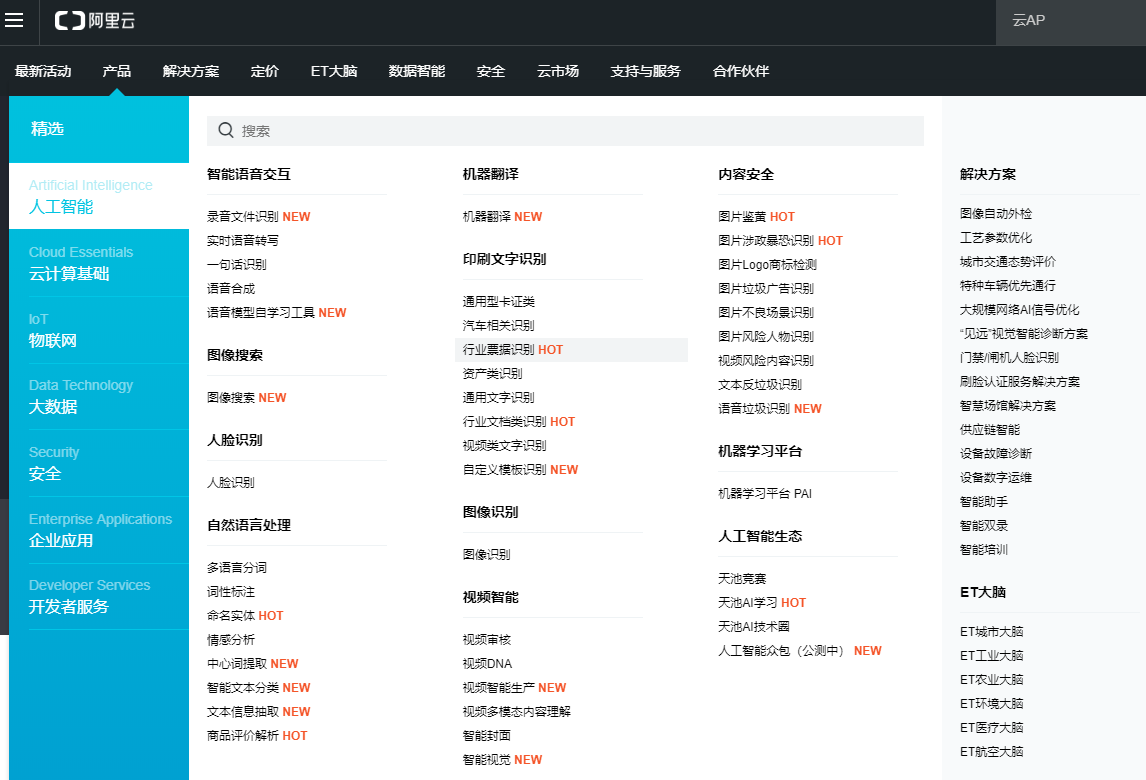
\includegraphics[width=0.4\columnwidth]{pic/chap1/aliyun.jpg}
    }
    \subfigure[谷歌云界面]{
        \label{fig:cloud_platform:b}
        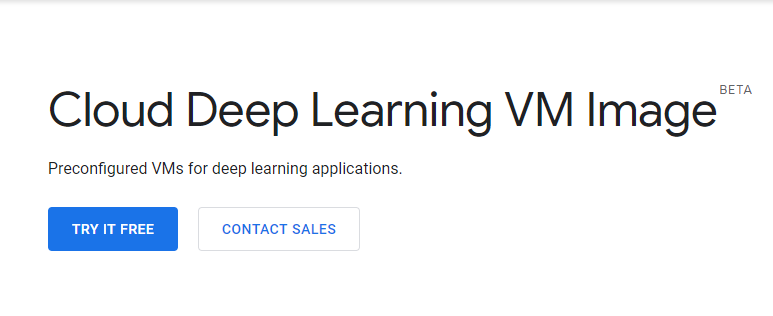
\includegraphics[width=0.4\columnwidth]{pic/chap1/googleyun.jpg}
    }
    \subfigure[亚马逊云界面]{
        \label{fig:cloud_platform:c}
        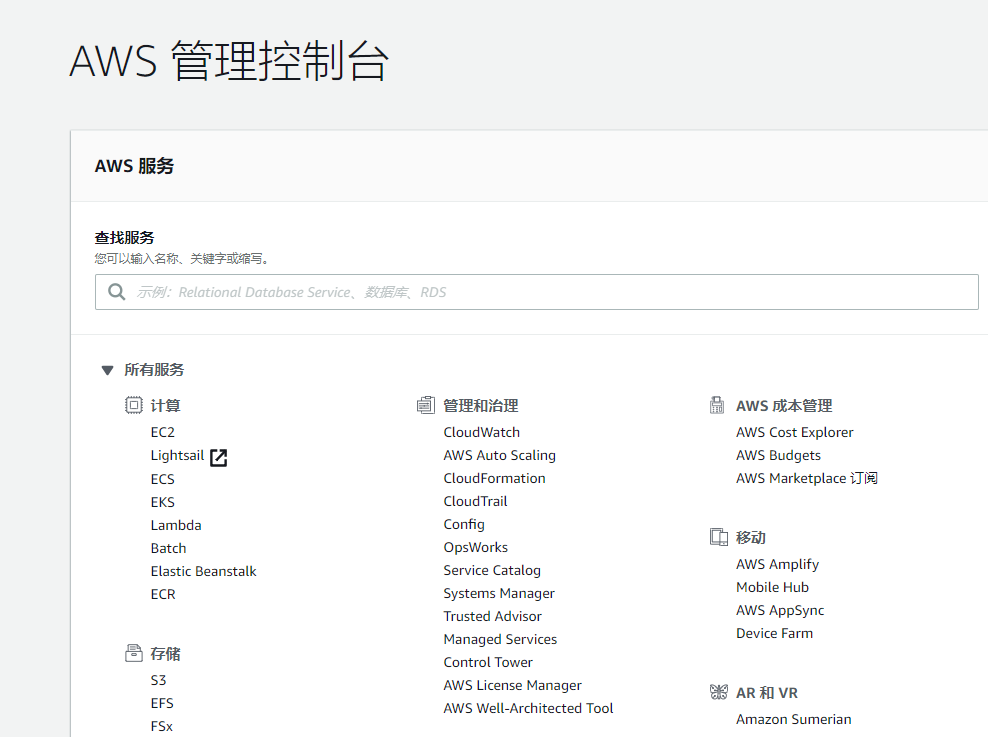
\includegraphics[width=0.4\columnwidth]{pic/chap1/AWSyun.jpg}
    }
    \subfigure[英伟达云界面]{
        \label{fig:cloud_platform:d}
        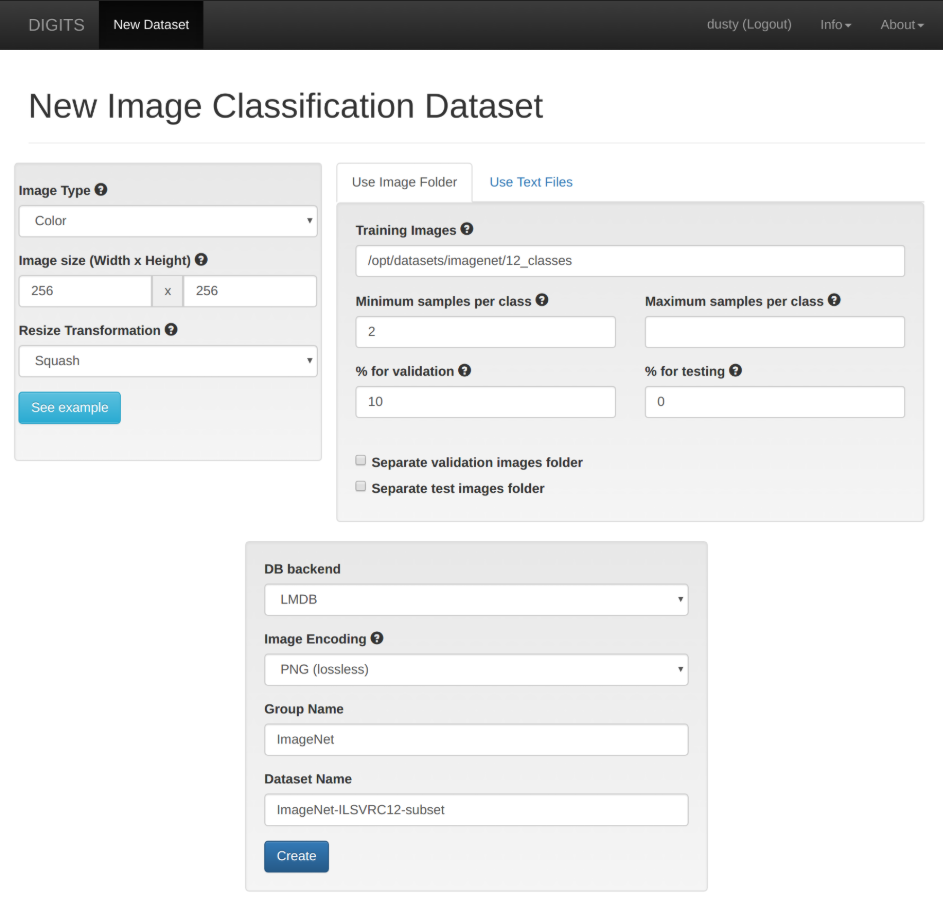
\includegraphics[width=0.4\columnwidth, height=0.3\columnwidth]{pic/chap1/nvidiayun.jpg}
    }
    \caption{国内外云平台实例}
    \label{fig:cloud_platform}
\end{figure}


国外云计算起步较早,如美国的谷歌、亚马逊、英伟达等公司均提供优秀的云服务。其中亚马逊云  \cite{AWSyun}占据了美国市场最大的份额。
亚马逊云界面如图\ref{fig:cloud_platform}\subref{fig:cloud_platform:c}所示。亚马逊云为客户提供功能十分丰富的云服务,其中,深度学习相关资源的提供方式和
阿里云类似。值得一提的是英伟达云(Nvidia GPU Cloud, NGC)    \cite{NVIDIAyun},其界面如图\ref{fig:cloud_platform}\subref{fig:cloud_platform:d},
NGC主要提供深度学习计算服务,并且与阿里云和亚马逊云只提供计算资源不同,NGC将常用的深度学习算法训练过程进行了封装,
通过网页端以选择框和文本框的形式供用户自定义深度学习训练参数配置。同时提供了常用的深度学习数据集供用户使用。用户只需要选择配置和数据集
即可训练自己的深度学习模型,大大降低了深度学习的计算和知识门槛。

综上可知,国内外云计算平台的深度学习服务主要通过API的方式提供,深度学习定制化模型一般只面向具备开发能力的开发者。而我国国内制造业从业者普遍缺乏云计算平台的使用能力
及深度学习知识,即使能够使用云计算提供的高计算资源,也很难去定制自身需要的深度学习模型。因此,针对国内制造业从业者缺乏深度学习知识而制造业又需要深度学习模型落地的具体
情况,开发一款面向制造业的封装良好且易于上手的云平台十分必要。


%%% 1.3 论文研究内容与架构
%%%%%%%%%%%%%%%%%%%%%%%%%%%%%%
\section{论文研究内容与架构}
\subsection{论文研究内容}
自动分拣系统主要由图像采集模块、图像处理模块和机器人模块构成,其中图像处理模块的核心为目标检测算法。传统的自动分拣系统,其主要采取传统的目标检测算法,针对
特定的检测工件,人工构造特征,进行模板匹配工件位置,然后使用这些特征作为分类器的输入再进行分类。总而言之,传统的分拣系统,其采取的目标检测算法需要根据不同
的工件人为构造特征,一旦工件发生变化,需要重新提取特征。这样的系统可移植性较差。随着深度学习的快速发展,基于神经网络的端到端的训练方式逐步改造着视觉方面的各类
算法。神经网络可以在训练过程中自动提取底层和高层特征,能够很好的表征图像特征,无需人为提取和构造特征,且效果也优于传统算法。由于神经网络的特征提取特性,
当工件类别发生变化时,无需耗费过多人力即可完成模型的移植,因此,基于深度学习的目标检测算法具有很好的可移植性。此外,基于国内制造业从业者缺乏深度学习知识和
技能的现状,业内急需一款面向制造业的低门槛深度学习云计算平台。出于以上几点,本论文设计并实验了一个基于深度学习目标检测算法的机械臂分拣系统,并开发了一个用于
定制深度学习目标检测模型的云平台。

本论文一共分为两部分。一是机械臂分拣系统的设计与实验;二是用于定制深度学习目标检测模型的云计算平台。

其中,基于深度学习的机械臂分拣系统需要实现如下功能或模块:
\begin{enumerate}
    \item{图像获取模块,实时获取图像信息,并以一定的通信方式将图片实时传递给图像处理模块。}
    \item{图像处理模块,接收图像获取模块传递来的图像信息,通过训练好的目标检测模型预测该图像中工件的位置及类别,并以一定的通信方式传递给机械臂模块。}
    \item{机械臂执行模块,包括机械臂控制模块和机械臂;接收当前图像中的工件位置和类别信息,将其转化为相应的控制指令,控制机械臂将工件抓起,并放到该工件类别相对应的位置。}
\end{enumerate}

定制深度学习目标检测模型的云计算平台需要实现以下功能:
\begin{enumerate}
    \item{Web端方面,提供文件上传功能,用于接收用户自行标注的数据集,以定制化目标检测模型。}
    \item{同样是Web端,以选择框或文本框的形式给出用户可自定义的超参数选项,方便用户定制化自己需要的模型特性。}
    \item{服务器端,接收Web端发送的各项参数,并根据参数执行相应的shell脚本,调用GPU训练深度学习目标检测模型,并且能够将训练过程中的各项参数实时同步到Web端,方便用户
    可视化模型的训练过程。}
\end{enumerate}

基于深度学习的目标检测模型虽然具有效果好、可移植性强等诸多优点,但其所需计算资源较大,难以在普通的嵌入式平台或台式机上运行,而使用GPU服务器进行实时计算会让整个系统显得
笨重,因此,如何在嵌入式平台进行深度学习模型的预测运算是一个难点。其次,图像采集模块、图像处理模块、机械臂控制模块需要高效的通信机制,以便以高FPS完成采集、处理、执行的流程。
云平台方面,则需要探究Web前端和服务器端的通信机制,及服务器端拿到配置信息后,如何调用GPU去训练深度学习模型。

针对以上问题,本论文针对以下方面进行了深入研究:
\begin{enumerate}
    \item{基于深度学习的目标检测模型的训练。首先搭建图像采集模块,并对所要检测的工件进行图像采集。针对这些图像,使用特定的图像标注工具进行标注。选取Yolov3作为目标检测模型,
    选取其开源框架Darknet进行训练,训练使用两块GTX 1080Ti显卡。并对其训练过程中的各项参数如Loss、IOU等值进行可视化分析。}
    \item{机械臂控制模块的设计实现。由于相机与机械臂所在空间的零点不一致,因此系统在使用之前需要进行标定。将机械臂和相机的坐标统一化。之后分析如何根据相机中工件的位置信息
    计算出机械臂下工件的位置信息,然后研究机械臂的控制方法,控制机械臂执行相应的动作。}
    \item{机器人通信机制研究。使用机器人操作系统(Robot Operation System,ROS)实现图像采集模块、图像处理模块、机械臂控制模块的高效通信。并研究如何将Yolov3模型封装为ROS节点,
    加入整个系统通信网络。}
    \item{云平台结构设计与实现。包括Web前端页面的设计与实现,文件上传功能的实现,使用JavaScript获取前端组件信息,并封装为JSON数据发送给服务端。服务端则需要接收并解析JSON配置数据,并编写相应的Linux
     shell脚本去训练定制化的深度学习模型,并将模型训练过程中的信息实时同步到Web前端。}
\end{enumerate}

\subsection{论文架构}
针对课题的研究内容,本论文各个章节的主要内容安排如下:

第1章,首先阐述了本论文的研究背景和研究意义;然后介绍了目标检测算法、基于视觉的自动分拣系统和深度学习云平台的国内外研究现状;最后给出了本论文的主要研究内容和论文架构。

第2章,主要从整体上阐述了本课题中基于深度学习的机械臂分拣系统的设计方案;并介绍了系统的硬件选型及依据,阐述了系统所使用的通信方案;之后根据本系统的具体条件,选择合适的
深度学习目标检测算法;最后介绍了如何进行相机标定和机械臂控制。

第3章,重点介绍图像处理模块。首先介绍了系统中使用的图像处理算法理论;然后介绍如何使用图像采集模块获取数据集并进行标注;最后是深度学习目标检测模型的训练、评估和部署。

第4章,首先介绍深度学习云平台的整体设计方案和通信方法,并进行了云平台的用户需求分析;之后分别介绍了云平台服务器端和Web端的实现方案。

第5章,分别就本论文的两大部分进行实验。第一部分对所选取的模型配置进行了实验,验证了YOLOv3-tiny模型配置针对本任务的优越性,并对自动分拣系统的延时和准确率进行了实验。第二部分则对深度学习
云平台服务端和Web端进行了稳定性测试实验。

第6章,对本论文所做的工作进行了总结,并对未来可作的改进工作进行了探讨。

论文的章节架构图如图    \ref{fig:paper_construct} 所示。

\begin{figure}
    \centering
    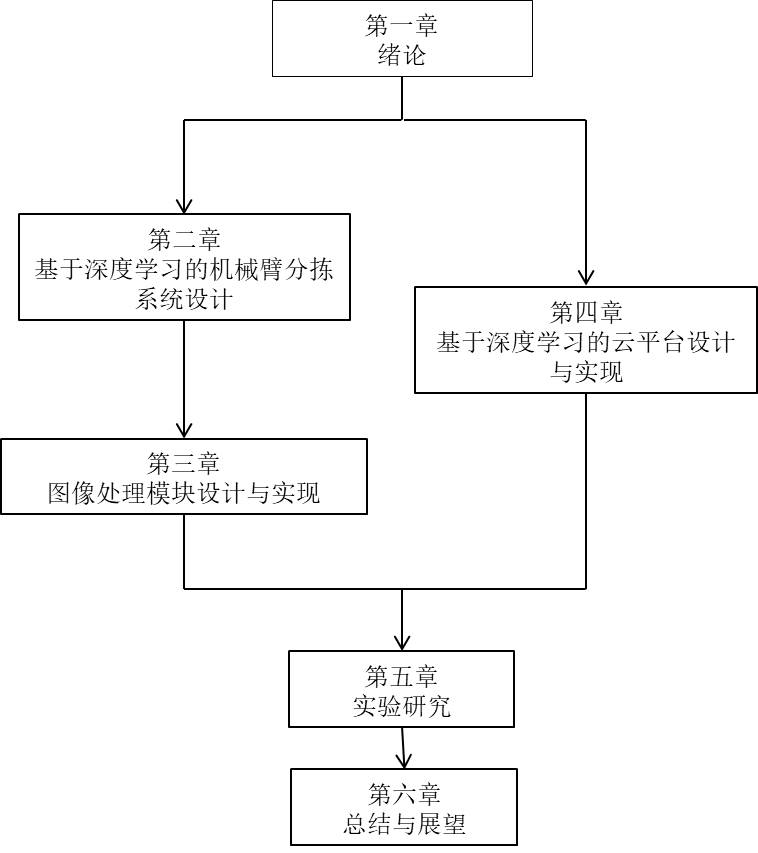
\includegraphics[scale=0.8]{pic/chap1/paper_construct.jpg}
    \caption{论文章节架构}
    \label{fig:paper_construct}
\end{figure}


\section{本章小结}
本章首先阐述了论文的研究背景和研究意义;然后介绍了目标检测算法、基于视觉的自动分拣系统和深度学习云平台的国内外研究现状;最后给出了本论文的主要研究内容和论文架构。
%%%%%%%%%%%%%%%%%%%%%%%%%%%%%%%
%%% 第二章 基于深度学习的机械臂分拣系统设计
%%%%%%%%%%%%%%%%%%%%%%%%%%%%%%%

\chapter{基于深度学习的机械臂分拣系统设计}

自动分拣系统的核心为图像处理模块,该模块的核心为目标检测算法。传统的目标检测算法需要人为为工件构造特征,
通过模板匹配的方式确定工件位置,再通过分类器的方式确定工件类别。当变换检测工件时,就需要针对工件再次构造特征。
而基于深度学习的目标检测算法则可以实现端到端的训练。这使得基于深度学习的机械臂分拣系统具有很强的可移植性。

自动分拣系统是一个多模块协同作用的系统。包括图像采集模块、图像处理模块和机械臂控制模块。这三个模块均建立在硬件
基础之上,且需要高效的通信机制。本章主要介绍整个自动分拣系统的整体架构和底层设计,包括硬件选型、通信流程等。然后
介绍了如何选择本系统中使用的目标检测算法,至于具体模型的介绍、训练及部署等,将放到第三章去讨论。最后,本章将介绍
目前相对已经比较成熟的相机标定及机械臂控制方法。

\section{系统整体架构}

系统的逻辑层面的架构图如图    \ref{fig:total_construct}
所示。

\begin{figure}[htbp]
    \centering
    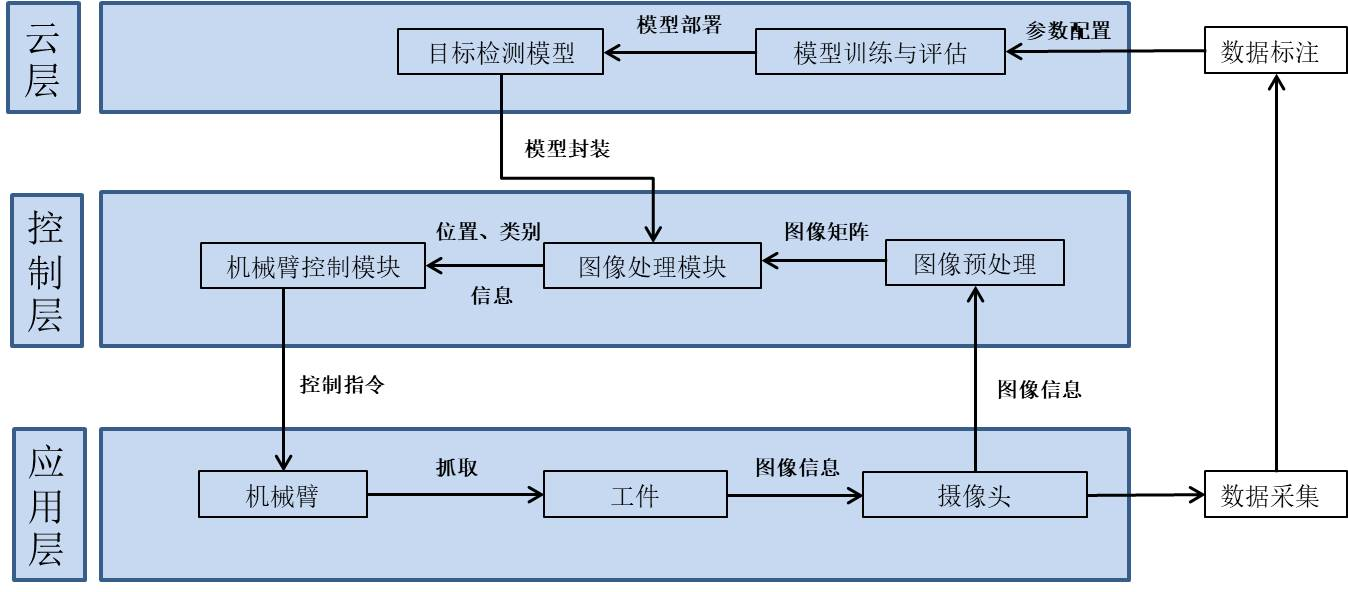
\includegraphics[width=\textwidth]{pic/chap2/total_construct.jpg}
    \caption{系统逻辑架构图}
    \label{fig:total_construct}
\end{figure}

基于深度学习的机械臂分拣系统逻辑上可以分为三个层面:应用层、控制层和云层(即服务器层)。以下对每个层面进行具体介绍:

1. 应用层

应用层由机械臂、工件和摄像头组成。主要是摄像头收集工件信息,机械臂对工件执行抓取动作。这一层面是整个系统对外展示的层面,
代表了整个系统的表现。

2. 控制层

控制层主要进行信息的处理和机械臂的控制指令生成。首先,控制层接收由应用层摄像头发送的图像信息,并进行预处理,之后发送给图像处理
模块中的目标检测模型进行预测,得到工件的位置和类别信息,然后发送给机械臂控制模块,由机械臂控制模块生成相应的机械臂控制指令,发送给
机械臂进行执行。

其中,摄像头和控制层的通信通过USB完成,所使用的摄像头为USB摄像头,主要是进行图像信息的传输;控制层和机械臂之间通过串口进行通信,
主要是进行机械臂控制指令的传输,如G代码等;而控制层的模块之间,则通过
机器人控制系统(Robot Operation System,ROS)进行,主要进行整型或浮点数的传输。

3. 云层(服务器层)

服务器层主要用于系统的搭建,在系统运行时是不参与工作的。服务器主要提供计算资源,用于深度学习模型的训练和评估。训练完成后,得到的其实是模型配置文件
和由大量浮点数组成的权重文件。模型配置文件主要用于描述模型的结构和参数,权重文件则用于描述模型网络的各个参数值。有了这些,就可以将模型部署和封装到
控制层,用于预测图像中工件的位置和信息。

此外,在三个层之外,还需要使用摄像头采集数据集,并进行标注,用作服务器层模型训练的数据集。

\section{系统硬件选型}

作为机械自动化及高性能计算一体的系统,基于深度学习的自动化分拣系统对硬件环境非常依赖。硬件性能的好坏将直接影响目标检测模型
的迭代次数、机械臂响应速度和分拣的延迟。因此,自动分拣系统的硬件选型非常重要。

本节主要介绍系统的硬件选型,包括用于采集图像信息的USB摄像头、用于高性能计算的服务器、运行图像处理模块和机械臂控制模块的
高性能嵌入式平台以及用于抓取工件的机械臂。

\subsection{相机}

\subsection{目标检测模型训练用服务器}

\subsection{目标检测运行硬件平台}

\subsection{机械臂选型}

\subsection{系统硬件架构}

\section{系统模块间通信机制}

\subsection{USB通信}

本系统中,USB通信主要用于摄像头向TX2传递图像信息。
本课题使用的USB版本为USB 3.0    \cite{USB3.0}版本,其传输速度为5Gbit/s,足以支撑高FPS的图像传输。

\subsection{ROS通信}

\subsection{串口通信}

\section{目标检测算法选型}

\section{相机标定及机械臂控制模块设计与实现}




%%% 第三章 机械臂抓取系统实现
%%%%%%%%%%%%%%%%%%%%%%%%%%%%%%%%
\chapter{图像处理模块设计与实现}
图像处理模块是自动分拣系统中的核心模块,关系着整个系统的性能表现。图像处理模块相当于自动分拣系统的“大脑”,
其中目标检测算法的预测用时将直接影响自动分拣系统的实时性,目标检测算法的准确率将直接影响自动分拣系统的分拣
准确率。因此,自动分拣系统的图像处理模块需要进行深入地研究和设计。本课题设计的自动分拣系统中的图像处理模块
使用了基于深度学习的目标检测算法和传统的计算图像相似度的图像算法,以便最大幅度提升图像处理模块的实时性,降低
系统延时。

本章主要介绍课题所设计的自动分拣系统中的图像处理模块,包括目标检测算法输入之前的图像预处理、基于深度学习的
目标检测算法的理论及其实际训练评估过程。最后介绍了如何将训练好的深度学习模型部署到Jetson TX2上,将其封装为
ROS节点,接入系统的通信网络。

\section{图像算法理论}
目标检测是计算机视觉领域的计算机技术,其涉及在数字图像和视频中检测特定对象的实例。目标检测算法应用十分广泛,
如人脸检测、人脸识别、对象跟踪等,当然,还有本论文中的工件识别。

基于深度学习的目标检测算法具有可移植性强、效果优异的优点,但深度学习模型一般具有海量的网络参数,
计算量大,运算效率不高。而自动分拣系统的场景下,并不是每一帧图像都需要输入目标检测算法进行工件
位置和类别的预测。一般情况下,只需要在机械臂执行之前进行预测。因此,本课题的图像处理模块,在图像信息
输入目标检测算法节点之前,加入了一个图像预处理节点,用于接收摄像头发送的图像信息,进行简单计算,判断
是否将该图像信息发送到目标检测算法节点。

本节将介绍课题中使用的两种图像算法:感知哈希算法\cite{ganzhihash}和YOLOv3。其中感知哈希算法用于图象预处理节点,用于判断工件是否处于
可抓取状态,若可抓取,则将图像发送到运行目标检测算法的节点进行处理,否则不进行处理。YOLOv3算法用于识别图像中
工件的位置和类别,为抓取提供信息。

\subsection{感知哈希算法}

自动分拣系统的场景中,我们希望机械臂抓取之前才进行目标检测步骤,以降低系统计算量,降低系统延时。本课题设计的自动分拣
系统,在工件静止时进行抓取,因此使用感知哈希算法来判断工件是否已经静止。感知哈希算法本身是用于图片相似度计算的算法,
可以通过计算前后几帧图片的相似度来间接判断图片是否静止。

感知哈希算法对每张图片生成一个“指纹”字符串,然后比较不同图片的指纹。结果越相近,说明图片越相似。其算法实习步骤如下:
\begin{enumerate}
    \item{第一步,缩小尺寸。
    
    将图片缩小到8×8的尺寸共64个像素点。这一步的目的是去除图片细节,只保留结构、明暗等基本信息。}
    \item{第二步,简化色彩。
    
    将第一步得到的图片,转化为64级灰度。即所有像素点只有64种灰度颜色。}
    \item{第三步,计算平均值。
    
    计算第二步得到的灰度图像的像素点平均值。}
    \item{第四步,比较像素灰度。
    
    将第二步得到的灰度图像中的像素点逐个与平均值比较,大于或等于平均值记为1,否则记为0。}
    \item{第五步,计算哈希值。
    
    将第四步的结果组合在一起得到一个64位的整数,这个整数就是图片的指纹。}
\end{enumerate}

对于输入的每张图片,可以通过以上方法得到该图片的“指纹”。对比不同的图片,计算64位整数中,有多少位是不一样的,即计算
它们的汉明距离\cite{hanming_distance}。若不同的数据位超过5位,说明两张图片很相似;若不同的数据位超过10位,则说明
这是两张不同的图片。

感知哈希算法的优点是非常的简单快速,不受图片大小缩放的影响。因此,可以用于图象预处理节点中,进行快速计算。此外,根据第三步
的不同,感知哈希算法又分为均值哈希算法和增强版的pHash\cite{pHash}。pHash引入了离散余弦变换\cite{DCT}(DCT)将图像从像素域
变换到频率域。该算法更加健壮,将均值的方法发挥到极致。本文使用的算法为pHash算法。

\subsection{YOLO}
YOLO是single-stage目标检测算法的代表。它将目标检测的问题处理为回归问题,用一个卷积神经网络就可以直接从一张输入
图像预测目标的位置和类别信息。

本文使用的基于深度学习的目标检测算法为YOLOv3。YOLOv3是YOLO(You Only Look Once)这个目标检测算法的第三个版本,
YOLOv3是YOLO算法的第三个版本,主要针对YOLO进行了一些细节的改进,因此,本小节主要介绍YOLO算法的原理。

YOLO的原理如图\ref{fig:YOLO_total}\cite{YOLO2016}所示,使用单个卷积神经网络预测每个物体的边界框和概率。YOLO训练全图像,并且直接
优化检测性能。与传统的检测方法相比,这种一步到位的模型具有以下优势:

\begin{figure}[htbp]
    \centering
    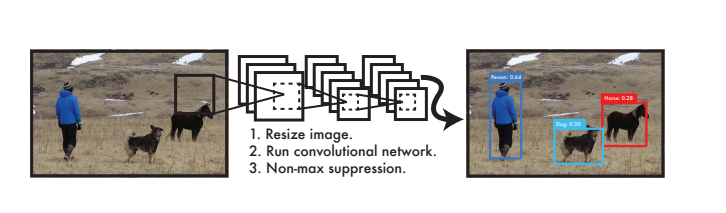
\includegraphics[scale=0.8]{pic/chap3/YOLO_total.jpg}
    \caption{YOLO目标检测系统}
    \label{fig:YOLO_total}
\end{figure}

\begin{enumerate}
    \item{YOLO非常快速。由于YOLO将目标检测问题简化为了回归问题,不再需要复杂的pipeline来进行特征提取和类别检测
    工作。}
    \item{与two-stage的目标检测算法不同,YOLO在预测时,使用了全局图像信息,因此能够显著降低错误率。}
    \item{由于YOLO端到端的训练特性,使得相比于R-CNN等检测算法,YOLO具有更强的可移植性。}
\end{enumerate}

YOLO使用整个图像的特征来预测每个目标的边界框(bounding boxes),可以同时预测所有类别的所有边界框。YOLO将输入图像
切分为S×S个网格,如果物体的中心落入某网格中,则该网格负责检测该物体。每个网格预测边界框和其置信度。边界框包括5个信息:
$x , y , w , h$和置信度。其中,$(x,y)$表示物体中心相对于网格单元框的坐标位置。$w,h$分别表示物体中心相对于整个
图像的宽度和高度。置信度则表示预测框和标注框的IOU(Intersection-Over-Union)值。模型逻辑如图\ref{fig:YOLO_model}所示。
每个网格预测$C$个条件概率,$Pr(Class_i|Object)$。
测试阶段,每个bounding box的置信度分数计算公式为:
\begin{equation}
    \centering
    \operatorname { Pr } \left( \text { Class } _ { i } | \text { Object } \right) * \operatorname { Pr } ( \text { Object } ) * \text { IOU } _ { \text { pred } } ^ { \text { truth } } = \operatorname { Pr } \left( \text { Class } _ { i } \right) * \text { IOU } _ { \text { pred } } ^ { \text { truth } }
    \label{YOLO_c}
\end{equation}

\begin{figure}[t]
    \centering
    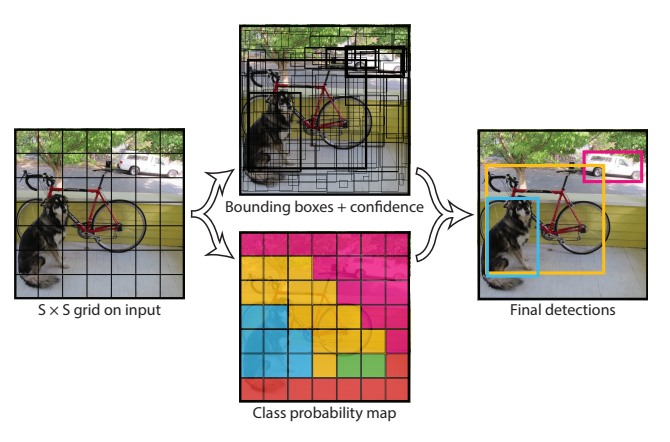
\includegraphics[scale=0.8]{pic/chap3/YOLO_model.jpg}
    \caption{YOLO模型逻辑}
    \label{fig:YOLO_model}
\end{figure}

\begin{figure} 
    \centering
    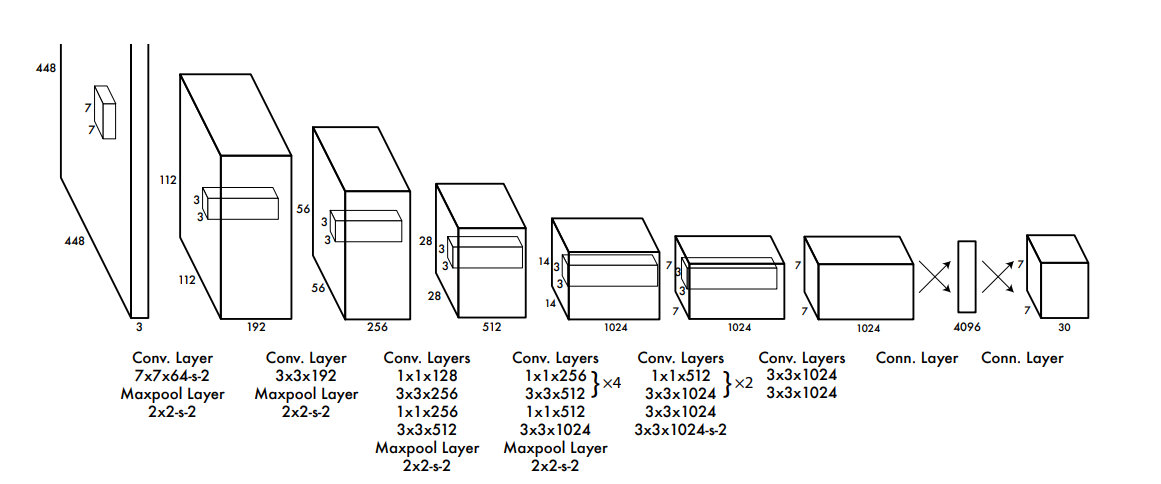
\includegraphics[scale=0.5]{pic/chap3/YOLO_construct.jpg}
    \caption{YOLO网络结构}
    \label{fig:YOLO_construct}
\end{figure}

在网络结构方面,YOLO使用卷积神经网络进行图片像素值到以上检测信息的映射。类似于GoogLeNet\cite{GoogLeNet2015},YOLO使用的网络结构为24层
卷积层后接两层全连接层。受Lin\cite{Lin}启发,YOLO将GoogLeNet初始模块中的3×3卷积层降维成1×1。整个网络结构如图\ref{fig:YOLO_construct}所示。


 
最后是模型的损失函数。由于目标检测需要预测目标物体的位置信息(即bounding box的信息)和类别信息,因此YOLO需要将两个任务的误差
损失结合到一个损失函数里面。YOLO采用sum-squared error的方式将bounding box的坐标误差和分类误差结合在一起。但如果两个任务的
损失权值一样,容易导致模型不稳定,不易收敛。因此采用对两个任务设置不同权重的方式。一方面,提高bounding box误差的权值,另一方面,
降低网格内部不包含物体中心的网格的分类损失权值。最终损失函数公式为:
$$\lambda _ { \text { coord } } \sum _ { i = 0 } ^ { S ^ { 2 } } \sum _ { j = 0 } ^ { B } 1 _ { i j } ^ { \mathrm { obj } } \left[ \left( x _ { i } - \hat { x } _ { i } \right) ^ { 2 } + \left( y _ { i } - \hat { y } _ { i } \right) ^ { 2 } \right]$$
$$+ \lambda _ { \text { coord } } \sum _ { i = 0 } ^ { S ^ { 2 } } \sum _ { j = 0 } ^ { B } 1 _ { i j } ^ { \mathrm { obj } } \left[ \left( \sqrt { w _ { i } } - \sqrt { \hat { w } _ { i } } \right) ^ { 2 } + \left( \sqrt { h _ { i } } - \sqrt { \hat { h } _ { i } } \right) ^ { 2 } \right]$$
$$+ \sum _ { i = 0 } ^ { S ^ { 2 } } \sum _ { j = 0 } ^ { B } 1 _ { i j } ^ { \mathrm { obj } } \left( C _ { i } - \hat { C } _ { i } \right) ^ { 2 }$$
$$+ \lambda _ { \mathrm { noobj } } \sum _ { i = 0 } ^ { S ^ { 2 } } \sum _ { j = 0 } ^ { B } 1 _ { i j } ^ { \mathrm { noobj } } \left( C _ { i } - \hat { C } _ { i } \right) ^ { 2 }$$
\begin{equation}
    \centering
    + \sum _ { i = 0 } ^ { S ^ { 2 } } 1 _ { i } ^ { \mathrm { obj } } \sum _ { c \in \text { classes } } \left( p _ { i } ( c ) - \hat { p } _ { i } ( c ) \right) ^ { 2 }
    \label{YOLO_J}
\end{equation}

其中,$1 _ { i } ^ { \mathrm { obj } }$表示网格$i$中是否存在物体的中心点; $1 _ { i j } ^ { \mathrm { obj } }$表示网格$i$预测的第$j$个
bounding box是否对该预测“负责”。$x , y , w , h$ 和 $C$的意义上文中已经进行了解释。
公式的前两行表示bounding box error,第一行表示网格中物体中心的坐标预测平方误差,第二行为宽度和高度预测的平方误差;第三、四行表示bounding box
的置信度损失,该损失分为网格内部是否落有物体中心分开计算。第五行代表分类误差。

总之,YOLO的思想,就是将目标检测问题通过设计合理的拟合对象和损失函数转换为回归问题。YOLO拟合的是图像像素值矩阵到bounding box和分类概率的映射
关系,通过最小化损失函数\ref{YOLO_J}得到最优的拟合关系。

\subsection{模型训练算法选择}

YOLO使用的网络结构为卷积神经网络,与通常的神经网络相同,其训练方法主要采用基于梯度下降的优化方法。
梯度下降法是优化领域最流行的算法,也是用于神经网络优化的最通用方法。它通过不断地
输入训练样本,朝着目标函数$J(\theta)$的负梯度的方向不断迭代网络参数$\theta \in \mathbb{R}^{d}$以优化
目标函数,逐步逼近最优参数解。学习率$\eta$表示每一步迭代的步长。

梯度下降法根据一次迭代使用多少数据可以分为
三个变种:批量梯度下降(Batch Gradient Descent,BGD)、随机梯度下降(Stochastic Gradient Descent,SGD)和
mini-batch梯度下降(mini-batch Gradient Descent,MBGD)。其中BGD使用所有数据进行一次迭代,SGD使用一个样本
进行一次迭代,MGD则介于两者之间,使用部分样本进行一次迭代。BGD的优点在于梯度计算准确,容易求得全局最优解,但需要消耗大量资源,并且
计算时内存不一定能加载所有数据;SGD使用的计算资源少,可以实现online-learning,但收敛速度慢。MBGD则是两者结合的产物。实际使用中,
一般使用MBGD。

然而,梯度下降法依然面临着许多问题,包括难以选取合适的学习率、避免陷入局部最优解等。为此,在梯度下降法的基础上,有许多算法
针对这些问题进行了优化。

\subsubsection{Momentum}
针对SGD在非凸优化问题中常见的“鞍点”问题,Momentum\cite{Momentum}可以帮助SGD在正确的方向上进行加速,而在不必要的方向上减少“震荡”。
Momentum通过将上一时刻更新矢量的$\gamma$倍添加到当前矢量上来实现:
$$v _ { t }  = \gamma v _ { t - 1 } + \eta \nabla _ { \theta } J ( \theta )$$
\begin{equation}
    \centering
    \theta  = \theta - v _ { t }
    \label{Momentum_F}
\end{equation}

\subsubsection{Adam}
Adaptive Moment Estimation(Adam)\cite{Adam}算法则是一个自适应学习率的梯度下降方法,它能够为每个网络参数自适应地
选择学习率。为了存储过去平方梯度的指数衰减平均值,Adam需要保存过去梯度$m_t$的指数衰减平均值:
$$m _ { t }  = \beta _ { 1 } m _ { t - 1 } + \left( 1 - \beta _ { 1 } \right) g _ { t }$$
\begin{equation}
    \centering
    v _ { t }  = \beta _ { 2 } v _ { t - 1 } + \left( 1 - \beta _ { 2 } \right) g _ { t } ^ { 2 } 
    \label{Adam_F_1}
\end{equation}

其中,$m_t$和$v_t$分别是梯度的第一时刻和第二时刻的估计值。同时,为了消除在初始时刻的偏差,通过如下公式更新$m_t$和$v_t$:
$$\hat { m } _ { t }  = \frac { m _ { t } } { 1 - \beta _ { 1 } ^ { t } } $$
\begin{equation}
    \centering
    \hat { v } _ { t }  = \frac { v _ { t } } { 1 - \beta _ { 2 } ^ { t } }
    \label{Adam_F_2}
\end{equation}
然后使用$m_t$和$v_t$来更新网络参数:
\begin{equation}
    \centering
    \theta _ { t + 1 } = \theta _ { t } - \frac { \eta } { \sqrt { \hat { v } _ { t } } + \epsilon } \hat { m } _ { t }
    \label{Adam_F_3}
\end{equation}

另外,与Adam类似的算法还有Adagrad\cite{Adagrad}、Adadelta\cite{adadelta}、RMSprop\cite{RMSprop}等算法,各个算法有各自的优势与劣势,下面一小节
中我们会对这些算法进行比较。

\subsubsection{优化算法比较与选择}
基于梯度下降法优化的各个算法,根据使用场景的不同,需要选择不同的算法。比如当输入数据比较稀疏时,使用自适应学习率的
方法不仅能取得最好的效果,同时也不需要调节学习率。总之,RMSprop是Adagrad的扩展,用以处理其急剧下降的学习率。它与Adadelta相同,
只不过Adadelta在更新规则中使用了参数更新的RMS。而Adam为RMSprop增加了偏差修正。RMSprop、Adadelta和Adam是非常相似的算法,
在类似的情况下表现良好。而随着梯度越来越稀疏,使用了偏差修正的Adam在训练的后期效果会更好。因此,Adam算法应该是大多数情况下
最优秀的训练算法。本课题在训练YOLOv3时使用的也是Adam算法。

\section{图像采集和数据获取}

任何模型,无论是深度学习模型还是传统的图像模型,第一步都是获取数据。数据是一切任务的前提,
只有有了数据,才能进行算法建模的下一步。因此,在训练深度学习目标检测模型之前,需要进行图像数据的
采集。这里使用ROS中的usb\_cam节点进行图像获取和数据采集。

由于我们使用的摄像头为USB摄像头,需要在ROS下安装USB驱动。安装之后,运行usb\_cam节点即可获取摄像头
的图像信息。由于训练模型需要的是图片数据,因此这里对usb\_cam节点源代码进行了更改,将实时视频的每一帧
图片保存到本地。同时,训练数据需要尽可能不同的图片,为了防止高FPS视频产生过多相同图片,这里将usb\_cam的
FPS从10降低到2,降低采样频率。更改方式为在usb\_cam.launch文件中加入如下配置:

$$ <param name="framerate" \quad value="2" />$$

同样为了降低图片的重复性,对视频图片进行随机降采样,即对每一帧图片,都以0.5的概率进行保存(或丢弃)。其具体公式
如下:

$$r = random(1)$$
\begin{equation}
    \centering
    IsSave =
        \begin{cases}
            1 & if \quad r >= 0.5\\
            0 & if \quad r < 0.5
        \end{cases}
\end{equation}

其中IsSave为usb\_cam节点的代码中的变量,当该变量为1时,将该帧图片保存到本地;否则对下一帧图片进行判断。

之后在摄像头固定的情况下,运行ROS的usb\_cam节点,将标注工件分别在摄像头下进行位置变换和角度变换等动作,从而
进行图片采集。采集的原则为,得到的图片集中要有单工件的不同位置和不同角度的图片,以及不同工件的共存图片。

\section{数据标注}

基于深度学习的目标检测模型属于监督学习,监督学习需要大量的有标注样本作为Ground Truth,通过标注样本计算损失函数的梯度,
然后使用Adam优化算法更新网络参数,直到损失函数得到最小值,网络得到最优解。因此,上一小节采集得到的图片需要进行标注。由于
YOLO模型是拟合图像像素矩阵值到bounding box和分类概率的映射关系,因此我们需要标注每张图像中工件的bounding box值,包括$x , y , w , h$,
以及该工件所属的类别。每张图片需要五个值。

\begin{figure}[h]
    \begin{minipage}{0.5\linewidth}
        \centering
        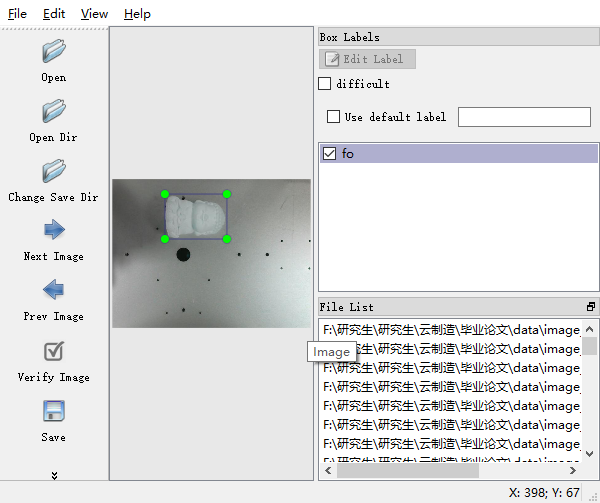
\includegraphics[scale=0.5]{pic/chap3/labelimg.jpg}
        \caption{LabelImg标注界面}
        \label{fig:LabelImg}
    \end{minipage}
    \begin{minipage}{0.5\linewidth}
        \centering
        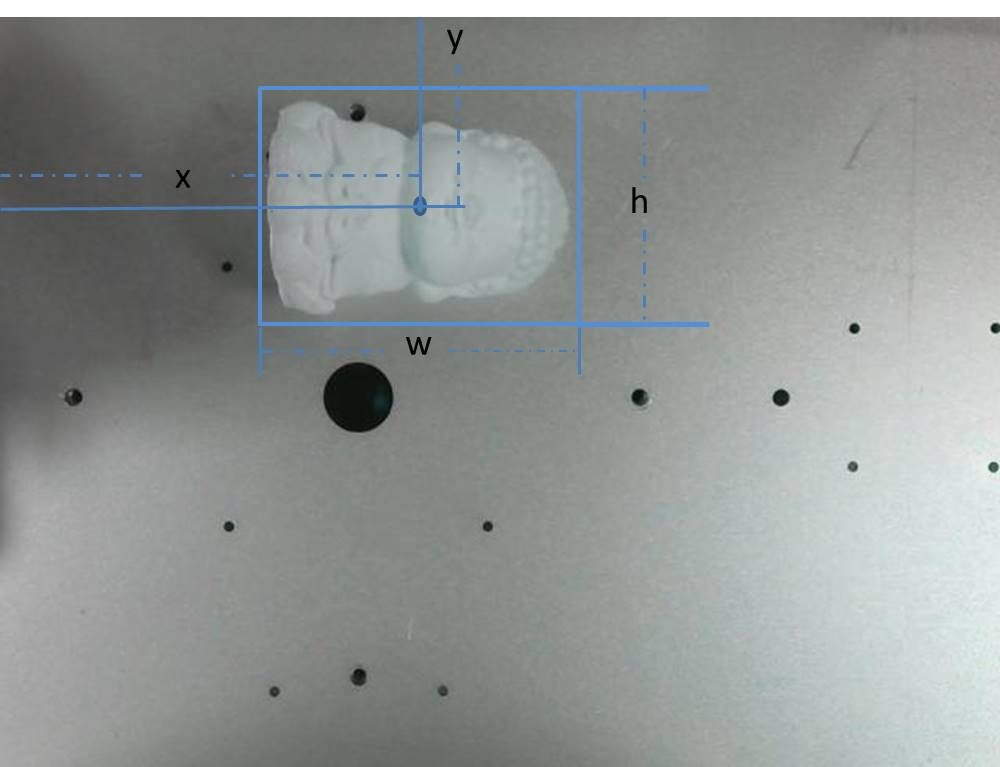
\includegraphics[scale=0.5]{pic/chap3/标注信息图示.jpg}
        \caption{标注信息图示}
        \label{fig:labelimg_info}
    \end{minipage}
\end{figure}

我们使用标注工具LabelImg \cite{LabelImg} 对采集到的图片数据进行标注,LabelImg标注界面如图 \ref{fig:LabelImg} 所示。每张图片标注并保存后会
生成一个与图片同名的txt文件,该文件内容如下(以其中一张图片为例):
$$1 \quad 0.420312 \quad 0.251042 \quad 0.312500 \quad 0.302083$$
该文件中一共5个值,分别代表物体的类别,$x , y , w , h$,其意义如表 \ref{table:LabelImg:info} 所示。在图片上的含义见图 \ref{fig:labelimg_info}。
{
    \begin{table}[htb]
        \zihao{5}
        \caption{标注数据含义}
        \label{table:LabelImg:info}
        \centering
        \begin{tabular}[t]{p{0.15\columnwidth} | p{0.15\columnwidth} | p{0.15\columnwidth} | p{0.15\columnwidth} | p{0.15\columnwidth}}
            \hline
            工件所属类别所占编号 & 工件中心横坐标x占整张图片宽度的比例 & 工件中心纵坐标y占整张图片高度的比例 & 边界框宽度w占整张图片宽度的比例 & 边界框高度h占整张图片的比例 \\
            \hline
            1 & 0.420312 & 0.251042 & 0.312500 & 0.302083\\
            \hline
        \end{tabular}
    \end{table}
}

最终共标注图片213张,产生213个txt文件。一共416个文件,构成了训练模型的标注数据集。将这些文件随机打乱之后,随机选取90\%作为训练数据集,剩下
10\%为测试数据集。

\section{目标检测模型训练与评估}
YOLO模型采用的网络结构为卷积神经网络,训练方法为基于梯度下降法的自适应学习率训练算法Adam。由于数据集图片数量不多,因此采用迁移学习的
方法来进行训练。此外,由于Jetson TX2计算能力有限以及需要检测的工件数量不多、特征明显,因此需要将YOLOv3的模型进行精简,以保证YOLOv3模型
部署在Jetson TX2上依然能够有足够的性能表现。

\subsection{模型评估方法}

首先介绍模型的评估方法。合理的评估方法能帮助我们合理的选择出最优的模型,从而取得最优的效果。

目标检测领域的评价体系中,最常用的评价指标为IOU(Intersection-Over-Union),同时,该参数也参与了Yolo损失函数的计算。因此,
本文选用IOU值作为评价模型的指标。

IOU即模型产生的目标窗口和标记窗口的重叠率。其公式如下:

\begin{equation}
    \centering
    I O U = \frac { \text { DetectionResult } \cap \text {GroundTruth} } { \text {DetectionResult} \cup \text {GroundTruth } }
    \label{IOU_equation}
\end{equation}

如图 \ref{fig:IOU_equation},IOU即图中蓝色区域面积除以所有图形面积之和。

\begin{figure}[htbp]
    \centering
    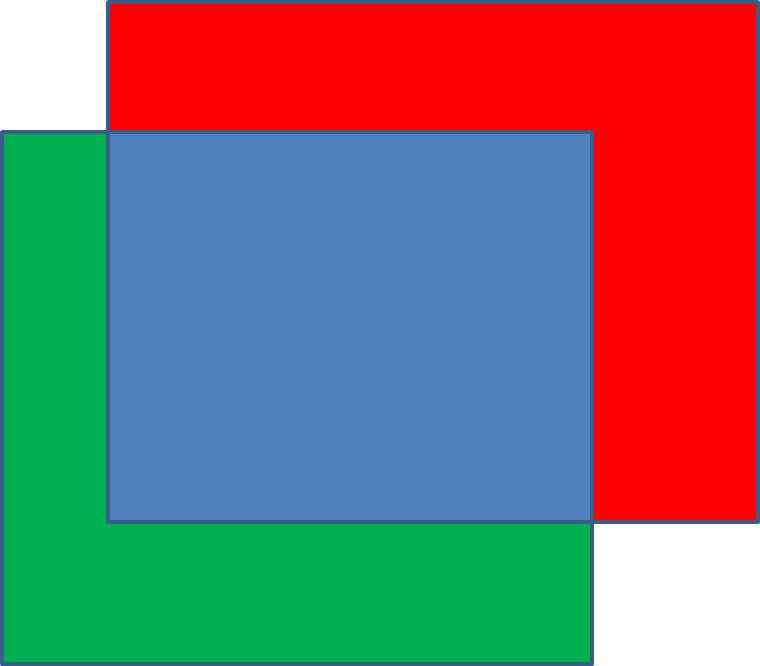
\includegraphics[scale=0.8]{pic/chap3/IOU.jpg}
    \caption{IOU计算方式图例}
    \label{fig:IOU_equation}
\end{figure}

\subsection{迁移学习}
机器学习是人工智能的重要方法。机器学习解决的是让机器自主地从数据中获取知识,从而应用于新的问题。而迁移学习作为机器学习的
一个重要分支,侧重于将已经学习过的知识迁移应用于新的问题。迁移学习的核心问题是如何找到新问题和原问题的相似性,只有找到
了相似性,才能将原问题学习到的知识应用到新问题上。使用机器学习的语言来说,迁移学习,是指利用数据、任务或模型之间的相似性,
将在旧领域学习过的模型,应用于新领域的一种学习过程。

迁移学习的研究主要是为了解决以下问题 \cite{TL_tutorial}:
 
\begin{enumerate}
    \item {大数据与少标注之间的矛盾。
    
    深度学习模型具有海量的参数需要训练,而这些训练都依赖于大量的标注数据。若标注
    数据过少,复杂的深度学习模型很容易陷入过拟合,而得不到好的训练结果。然而数据的标注
    是一个耗时且昂贵的操作,因此深度学习需要大量标注数据与数据标注的困难形成了一个矛盾。
    通过寻找与目标数据相近的有标注数据,利用这些数据来构建模型,增加目标数据的标注。迁移
    数据标注的方式可以有效解决这种问题。}
    \item {大数据与弱计算之间的矛盾。
    
    深度学习模型一般需要海量的计算资源,如NLP界的巨无霸模型BERT\cite{BERT}模型,谷歌
    使用了16个TPU集群(共64块TPU)训练了四天。而大部分开发者是无法触及这么大规模的计算资源
    的。利用迁移学习的思想,我们可以使用那些已经在大数据上训练好的模型,迁移到自己的任务中,
    针对自己的任务进行微调,从而获得更好的模型效果。}
\end{enumerate}

\begin{figure}[htbp]
    \centering
    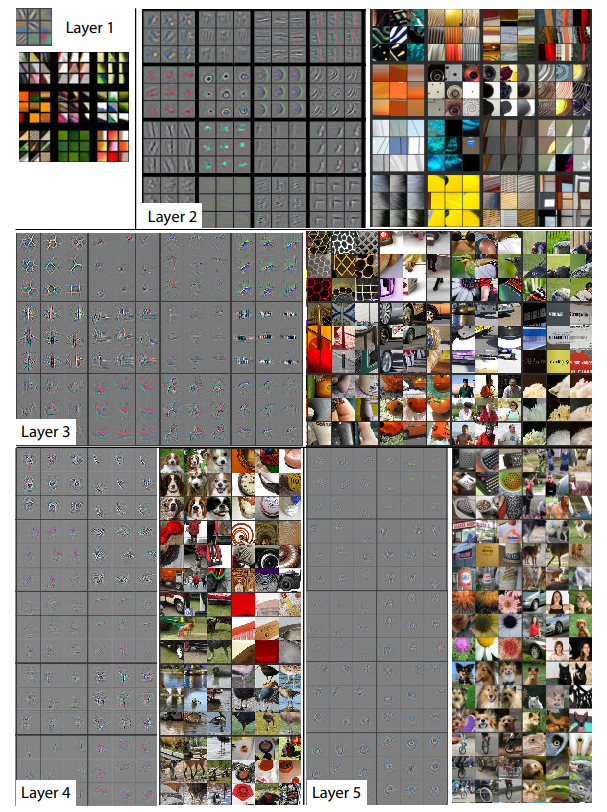
\includegraphics{pic/chap3/imagenet_vis.jpg}
    \caption{卷积神经网络中间层特征可视化}
    \label{fig:ImageNet:vis}
\end{figure}
 
表 \ref{table:TL:biyao} 展示了迁移学习的必要性。
{
    \begin{table}[htb] 
        \zihao{5}
        \caption{迁移学习的必要性}
        \label{table:TL:biyao}
        \centering
        \begin{tabular}[t]{c|c|c}
            \hline
            矛盾 & 传统机器学习 & 迁移学习 \\
            \hline
            大数据与少标注 & 增加人工标注,耗时且昂贵 & 数据的迁移标注\\
            \hline
            大数据与弱计算 & 只能依赖强大的计算能力 & 模型迁移\\
            \hline
        \end{tabular}
    \end{table}
}

在图像领域,通常作为迁移学习的基模型的为Google在ImageNet数据集上预训练的模型。ImageNet
是目前世界上图像识别最大的数据库。在ImageNet上训练得到的神经网络模型,其中间层一般都具有
表征图像底层或高层特征的能力。如图 \cite{ImageNet_vis} \ref{fig:ImageNet:vis} ,在ImageNet上训练得到卷积神经网络,其底层抽取出
边缘角点以及颜色特征,越到高层越呈现出具体的特征。由于预训练得到的网络参数,已经具备了表征图像特征的能力,因此
从这些网络参数出发,在特定的图像任务上,已经比较接近最优解,只需要在特定任务的小数据集上进行再次训练,即可
达到该任务下的最优解。



在本文中,将选用在ImageNet预训练的YOLO模型作为迁移学习的基模型,即使用在大数据集上预训练得到的网络
参数作为本任务的网络初始参数,然后使用本任务的数据集上继续迭代参数,直到网络收敛。






\subsection{模型训练}
结合自动分拣系统的硬件实际情况,本课题一共训练了两种YOLOv3模型,两种模型除网络配置外,其余所有情况包括
数据集、训练方法等均相同。第一种使用论文作者的原始配置,称为YOLOv3,另一种则将网络结构进行了精简,使用了更少
的网络参数,叫做YOLOv3-tiny。表 \ref{table:model:config} 展示了两种模型配置的不同之处。

{
    \begin{table}[htb] 
        \zihao{5}
        \caption{YOLOv3和YOLOv3-tiny配置参数比较}
        \label{table:model:config}
        \centering
        \begin{tabular}[t]{c|c|c|c|c|cc|c|c|c}
            \hline
            配置 & batch & width & height & 卷积层数 & 池化层数  \\
            \hline
            YOLOv3 & 16 & 640 & 480 & 75 & 0 \\
            \hline
            YOLOv3-tiny & 16 & 640 & 480 & 13 & 6 \\
            \hline
            配置 & shortcut(Res)层数 & unsample层数 & Route层数 & yolo层数\\
            \hline
            YOLOv3 & 23 & 2 & 4 & 3\\
            \hline
            YOLOv3-tiny & 0 & 1 & 2 & 2\\
            \hline
        \end{tabular}
    \end{table}
}

其中,batch为训练过程中每迭代一次参数使用的样本数量;width和height为所使用的训练图片的宽度和高度;卷积层数为神经网络结构中,卷积层
的数量;池化层数为网络中使用的最大池化层(max-pooling)的数量;shortcut层类似于ResNet \cite{ResNet}中的残差连接,用于将底层特征传输到高层;
upsample层的作用是对前一层的特征进行上采样;Route层用于索引特征图;yolo层为检测层。

使用的迁移学习基模型也是基于上述两种配置在ImageNet上预训练得到的网络参数。使用YOLO的开源训练框架DarkNet \cite{DarkNet}
进行训练。训练过程中的参数情况如图 \ref{fig:train:log} 所示。
\begin{figure}[h]
    \centering
    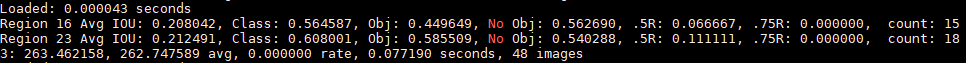
\includegraphics[width=\textwidth]{pic/chap3/train_log.png}
    \caption{训练过程参数示意图}
    \label{fig:train:log}
\end{figure}

\begin{figure}[t]
    \centering
    \subfigure[Loss曲线图 Batch:0-2000]{
        \label{fig:Loss:fullbatch}
        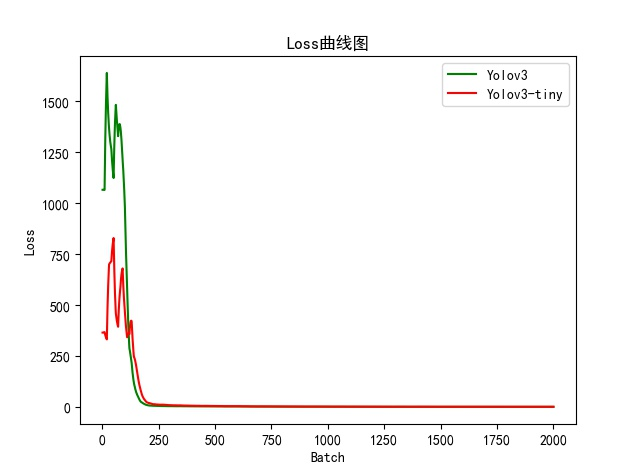
\includegraphics[width=0.46\columnwidth]{pic/chap3/Loss-v3&v3_tiny.jpeg}
    }
    \subfigure[Loss曲线图 Batch:500-2000]{
        \label{fig:Loss:partbatch}
        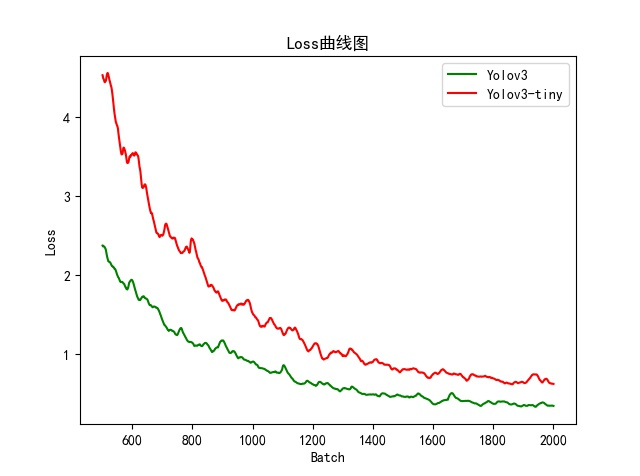
\includegraphics[width=0.46\columnwidth]{pic/chap3/Loss-v3&v3_tiny-scaled.jpeg}
    }
    \caption{Yolov3和Yolov3-tiny的Loss曲线对比图}
    \label{fig:Loss}
\end{figure}

\begin{figure}[t]
    \centering
    \subfigure[IOU曲线图 Batch:0-2000]{
        \label{fig:IOU:fullbatch}
        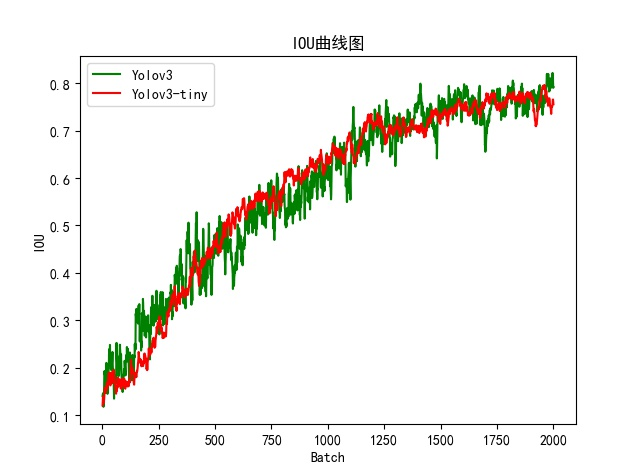
\includegraphics[width=0.46\columnwidth]{pic/chap3/IOU-v3&v3_tiny.jpeg}
    }
    \subfigure[IOU曲线图 Batch:500-2000]{
        \label{fig:IOU:partbatch}
        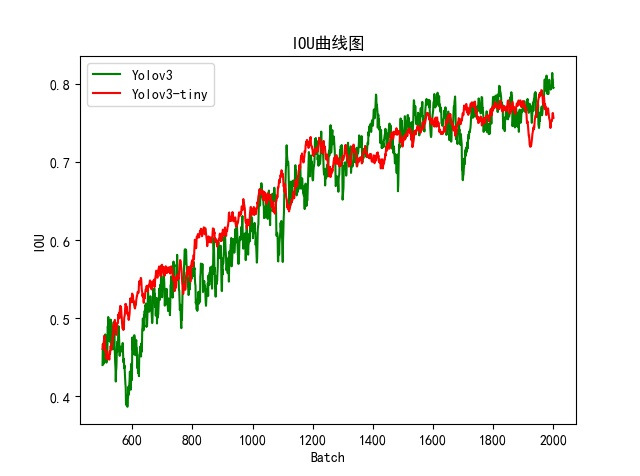
\includegraphics[width=0.46\columnwidth]{pic/chap3/IOU-v3&v3_tiny-scaled.jpeg}
    }
    \caption{Yolov3和Yolov3-tiny的IOU曲线对比图}
    \label{fig:IOU}
\end{figure}

图 \ref{fig:train:log} 显示了所有训练图片的一个批次(batch)。图片的第一行表示该批次训练所用时间。剩下的输出包括批输出
和分块输出。该图的批输出如下:
$$3: \quad 263.462158,\quad 262.747589 \; avg,\quad  0.000000 \; rate, \quad 0.077190 \; seconds, \quad 48 \; images$$

其中3表示当前训练的迭代次数;263.462158代表总体的Loss;262.747589 avg表示平均Loss,越低越好;
0.000000 rate表示当前的学习率;0.077190 seconds表示当前批次花费的总时间;48 images表示到目前为止训练的图片的总数量。

\begin{figure}[h]
    \centering
    \subfigure[Loss曲线图 Batch:0-2000]{
        \label{fig:Loss-TL:fullbatch}
        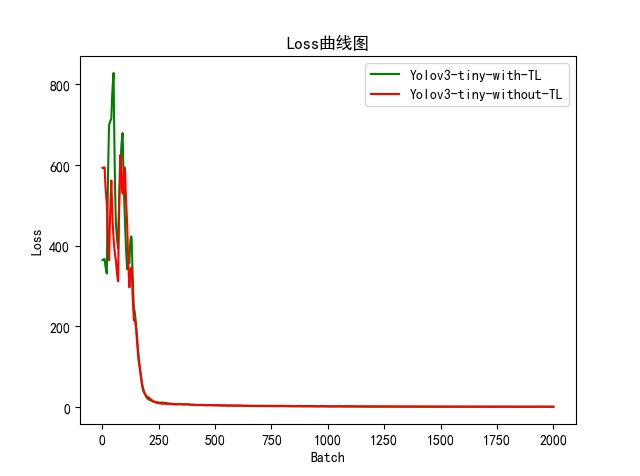
\includegraphics[width=0.46\columnwidth]{pic/chap3/Loss-v3_tiny&v3_tiny_noTL.jpeg}
    }
    \subfigure[Loss曲线图 Batch:500-2000]{
        \label{fig:Loss-TL:partbatch}
        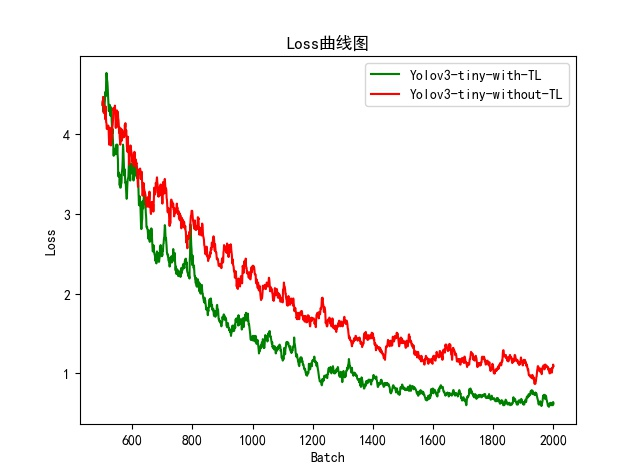
\includegraphics[width=0.46\columnwidth]{pic/chap3/Loss-v3_tiny&v3_tiny_noTL-scaled.jpeg}
    }
    \caption{Yolov3-tiny是否使用迁移学习的Loss曲线对比图}
    \label{fig:Loss_TL}
\end{figure}


\begin{figure}[h]
    \centering
    \subfigure[IOU曲线图 Batch:0-2000]{
        \label{fig:IOU-TL:fullbatch}
        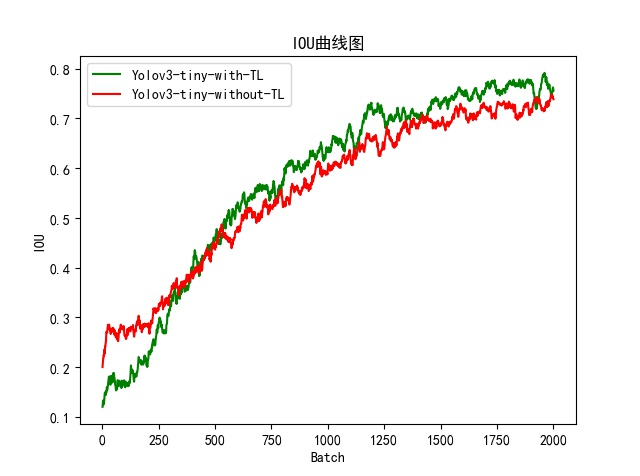
\includegraphics[width=0.46\columnwidth]{pic/chap3/IOU-v3_tiny&v3_tiny_noTL.jpeg}
    }
    \subfigure[IOU曲线图 Batch:500-2000]{
        \label{fig:IOU-TL:partbatch}
        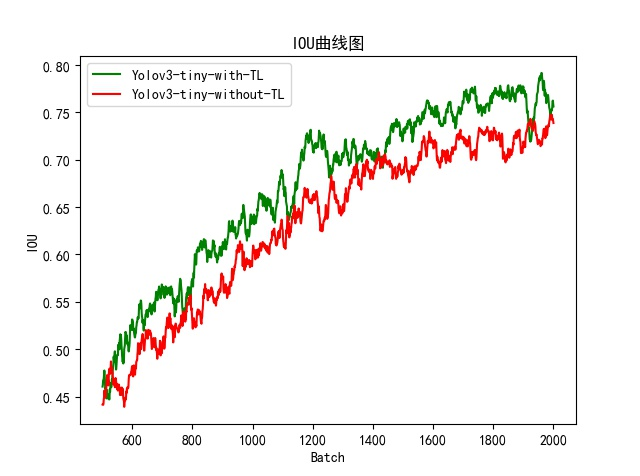
\includegraphics[width=0.46\columnwidth]{pic/chap3/IOU-v3_tiny&v3_tiny_noTL-scaled.jpeg}
    }
    \caption{Yolov3-tiny是否使用迁移学习的IOU曲线对比图}
    \label{fig:IOU_TL}
\end{figure}

该图的分块输出如下:
$$Region\;23 \quad Avg IOU: 0.212491, \  Class: 0.608001, \  Obj: 0.585509, \  No Obj: 0.540288, $$
$$\ .5R: 0.111111, \ .75R: 0.000000, \  count: 18$$

上述参数中,Region 23 Avg IOU表示在当前分区内,图片的平均IOU,表示预测的矩形框和真实目标框的交集与并集之比。这里是21.25\%;Class:0.608001表示标注物体
的分类正确率,该值趋近于1;Obj: 0.585509表示把正样本判断为正样本的平均置信度为0.59,该值期望趋近于1;No Obj则期望趋近于0;.5R和.75R分表表示当前模型
在所有分块中检测出的正样本数量与实际的正样本数量的比值,全部样本被检测到这两个值均为1;count则表示所有分块的图片中
包含正样本的图片的数量。

训练过程中,在达到不同的batch数节点时会进行权重的保存。具体来说,前1,000个batch,每100个batch会进行一次权重的保存;之后每10,000个batch进行一次权重
文件保存。当平均损失降低到0.2以下时即可结束训练。最后选择平均IOU最高的权重文件作为最终使用的网络参数。


\begin{figure}[t]
    \centering
    \subfigure[预测用时曲线图]{
        \label{fig:inf_time:curve}
        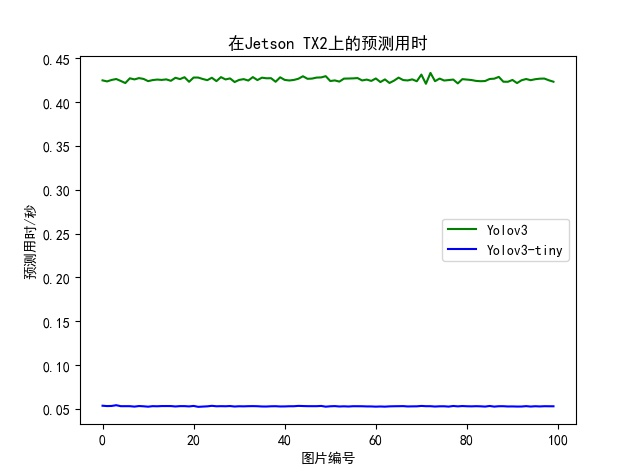
\includegraphics[width=0.46\columnwidth]{pic/chap3/time-v3&v3_tiny.jpeg}
    }
    \subfigure[预测平均用时柱状图]{
        \label{fig:inf_time:bar}
        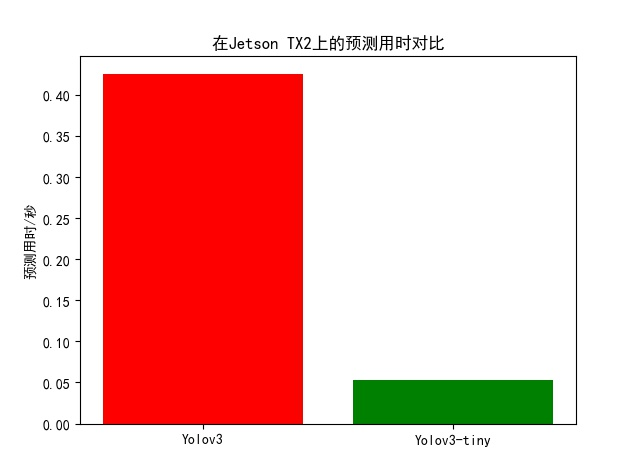
\includegraphics[width=0.46\columnwidth]{pic/chap3/time-v3&v3_tiny-avg.jpeg}
    }
    \caption{Yolov3和Yolov3-tiny的预测用时对比}
    \label{fig:inf_time}
\end{figure}

\begin{figure}[t]
    \centering
    \subfigure[模型预测效果1]{
        \label{fig:model_pre:1}
        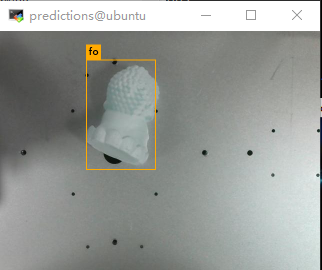
\includegraphics[width=0.46\columnwidth]{pic/chap3/model_prediction_1.png}
    }
    \subfigure[模型预测效果2]{
        \label{fig:model_pre:bar}
        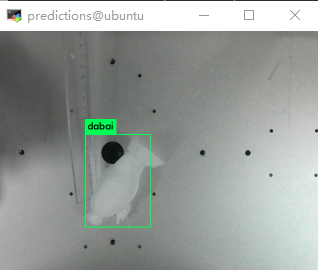
\includegraphics[width=0.46\columnwidth]{pic/chap3/model_prediction_2.png}
    }
    \caption{模型预测效果示意图}
    \label{fig:model_pre}
\end{figure}


Yolov3和Yolov-tiny模型训练过程的Loss变化曲线如图 \ref{fig:Loss} 所示。整体来看,经过2000个Batch,两个模型收敛的速度
及达到的损失函数值非常接近。Yolov3最终的Loss值略低于Yolov3-tiny。两个模型训练过程中的IOU变化曲线如图 \ref{fig:IOU} 所示。
两个模型的IOU变化及最终达到的IOU值相似。由上述两幅图可知,针对该任务,Yolov3-tiny和Yolov3的效果表现类似。而两者在Jetson TX2进行
模型预测的用时情况如图 \ref{fig:inf_time} 所示,由图可知,Yolov3-tiny在Jetson TX2上的预测用时远远小于Yolov3,说明了本任务选用Yolov3-tiny模型配置
的优势。

同时,在基于ImageNet预训练模型训练之外,本文也训练了不使用迁移学习的模型,以论证迁移学习的必要性和有效性。如图 \ref{fig:Loss_TL},是否使用迁移学习
模型的训练过程Loss曲线对比显示,使用迁移学习的Yolov3-tiny模型,在经过2000个Batch的训练后,取得了比不使用迁移学习的Yolov3-tiny模型更低
的Loss值。IOU方面,如图 \ref{fig:IOU_TL},IOU对比曲线显示,使用迁移学习的Yolov3-tiny模型,取得了更高的IOU值。这两幅图充分说明了基于本任务
选用基于ImageNet预训练的模型进行迁移学习的必要性。

通过对比,本论文最终选用基于迁移学习的Yolov3-tiny模型,作为自动分拣系统的目标检测算法进行使用。模型预测效果如图 \ref{fig:model_pre} 所示。
由图可知,模型可以准确的预测出目标物体的边框和类别。

\section{目标检测模型部署}

目标检测模型训练好之后,只能用于测试图片文件查看效果,并不能实际应用。因此,需要将训练好的Yolo目标检测模型进行封装,
将其作为一个ROS节点,加入自动分拣系统的ROS通信网络,以便被其他模块调用。

本文使用darknet\_ros \cite{darknet_ros}对模型进行封装。将darknet\_ros配置到Jetson TX2上之后进行编译,然后根据
本任务进行配置。主要包括模型权重文件和配置文件替换、ROS相关配置和启动项配置。配置好之后,启动yolov3.launch节点,
即可使用之前训练好的模型进行检测,并将边框和类别信息发布到/darknet\_ros/boundingboxes话题下,其余模块可通过订阅
该话题来接收物体的类别和边框信息。

\section{本章小结}
本章主要介绍图形处理模块。本文的自动分拣系统使用了传统的图像算法和基于深度学习的目标检测算法,本章介绍了所使用
的算法的原理。然后介绍了得到目标检测算法模型的流程,包括数据获取、数据标注、模型的训练和评估方法。然后选择了
使用迁移学习的Yolov3-tiny配置模型进行实际应用。最后介绍了如何将训练好的模型部署到ROS的通信节点中。
\chapter{基于深度学习目标检测模型的云平台设计与实现}

\section{深度学习云平台方案设计}

\subsection{云平台整体架构}

\subsection{基于Http协议的通信方法分析}

\subsection{云平台性能需求分析}

\section{基于Flask的Web服务端设计与实现}

\subsection{云平台服务端架构}

\subsection{基于Linux的Shell脚本实现云平台模型训练}

\section{基于Web前端的客户端系统设计}

\subsection{客户端网页需求分析}

\subsection{客户端页面分析、设计与实现}

\subsection{Web前端与服务器端的通信实现}



\chapter{实验研究}

本章主要通过实验来验证所选用硬件组成自动分拣系统的可用性、稳定性和准确定,以及所选用目标检测算法的优越性。然后通过实验
验证深度学习云平台的可用性与稳定性。第一部分将针对自动分拣系统的分拣延时和分拣准确率进行实验,对YOLOv3和YOLOv3-tiny在
自动分拣系统中的延时进行对比与选择。然后对应用YOLOv3-tiny的自动分拣系统的分拣准确率进行实验。第二部分针对深度学习云平台的
Web前端和服务器后端进行了性能稳定性测试。

\section{机械臂分拣系统性能实验}

本节将所设计的基于深度学习的自动分拣系统进行实验,包括图像处理模块的延时实验和分拣准确率实验。其中,延时实验主要是将YOLOv3和YOLOv3-tiny
部署在自动分拣系统后的延时进行对比,从而验证选择YOLOv3-tiny模型配置的优越性。分拣准确率实验又包括
分拣分类准确率实验和抓取成功率实验。前者主要衡量图像处理模块将工件进行准确分类的能力,后者主要衡量图像处理模块识别工件边框
的能力。

本实验中,硬件平台如表\ref{table:exper:hardware}所示。

{
    \begin{table}[htb] 
        \zihao{5}
        \caption{实验各硬件平台配置表}
        \label{table:exper:hardware}
        \centering
        \begin{tabular}[t]{c|c|c|c|c|c}
            \hline
            工件 & 摄像头 & 图像处理平台 & 机械臂 & 显示器 & 服务器  \\
            \hline
            3D打印工件 & 罗技C270 & Jetson TX2 & DOBOT & AOC I2490VXH & DELL T630 \\
            \hline 
        \end{tabular} 
    \end{table}
}

上表所示配置即第二章中所介绍的自动分拣系统的硬件选型配置。实验环境下为自动分拣系统的Jetson TX2配备了显示器,
主要目的为观测目标检测的效果实况,以及记录当前图像处理的FPS。此外,实验环境和实际使用中,Jetson TX2开启最大功耗模式。

软件环境如表\ref{table:exper:software}所示。

{
    \begin{table}[htb] 
        \zihao{5}
        \caption{实验软件环境配置表}
        \label{table:exper:software}
        \centering
        \begin{tabular}[t]{c|c|c|c|c|c}
            \hline
            操作系统 & 模块通信 & G-Code支持 & 算法部署 & 编译工具 & 脚本环境  \\
            \hline
            Linux tegra-ubuntu & USB/ROS/串口 & Marlin固件 & darknet\_ros & catkin\_make & Python/Shell \\
            \hline 
        \end{tabular} 
    \end{table}
}

分拣延时的实验数据通过修改自动分拣系统图像处理模块代码直接将数据保存到本地得到;分拣准确率的实验数据通过人工放置工件和人工观察记录得到。


\subsection{自动分拣系统图像处理模块算法性能试验}

本文第三章第三节中已对YOLOv3和YOLOv3-tiny的性能进行了比较,该比较基于服务器环境,非部署环境。因此本小节将对部署后两者的性能进行对比试验,以
验证针对本任务YOLOv3-tiny配置的优越性。

使用darknet\_ros分别将YOLOv3和YOLOv3-tiny配置的模型部署到自动分拣系统的图像处理模块进行延时实验。实验比较参数为FPS(Frame per Second),即图像处理模块预测图片后显示到显示器
上的帧率。该参数可以反映出图像处理模块进行图像预测的能力,即每秒能够处理的图片数量。实验采集了两个模型部署后处理图片的50个瞬时FPS数据,
数据采集如表\ref{table:delay:data}所示。

{
    \begin{table}[htb] 
        \zihao{5}
        \caption{延时实验数据采集表}
        \label{table:delay:data}
        \centering
        \begin{tabular}[t]{c|c|c|c|c|c|c|c|c|c|c}
            \hline
            \diagbox{配置}{FPS}{编号} & 1 & 2 & 3 & 4 & 5 & 6 & 7 & 8 & 9 & 10 \\
            \hline
            YOLOv3 & 1.51 & 1.48 & 1.49 & 1.53 & 1.56 & 1.50 & 1.54 & 1.55 & 1.40 & 1.48\\
            %%\hline 
            YOLOv3-tiny & 14.92 & 15.20 & 15.49 & 14.65 & 14.90 & 14.78 & 14.56 & 15.50 & 15.18 & 15.04\\
            \hline
            & 11 & 12 & 13 & 14 & 15 & 16 & 17 & 18 & 19 & 20 \\
            \hline
            YOLOv3 & 1.49 & 1.54 & 1.52 & 1.54 & 1.51 & 1.40 & 1.44 & 1.49 & 1.47 & 1.52\\
            %%\hline 
            YOLOv3-tiny & 15.41 & 15.10 & 15.19 & 15.65 & 14.98 & 15.12 & 15.34 & 14.90 & 14.88 & 14.72\\
            \hline
            & 21 & 22 & 23 & 24 & 25 & 26 & 27 & 28 & 29 & 30 \\
            \hline
            YOLOv3 & 1.38 & 1.46 & 1.42 & 1.52 & 1.54 & 1.44 & 1.53 & 1.45 & 1.50 & 1.52\\
            %%\hline 
            YOLOv3-tiny & 15.01 & 15.22 & 15.05 & 15.43 & 14.87 & 15.23 & 15.04 & 14.81 & 14.78 & 14.92\\
            \hline
            & 31 & 32 & 33 & 34 & 35 & 36 & 37 & 38 & 39 & 40 \\
            \hline
            YOLOv3 & 1.49 & 1.50 & 1.56 & 1.42 & 1.50 & 1.41 & 1.43 & 1.53 & 1.55 & 1.51\\
            %%\hline 
            YOLOv3-tiny & 14.91 & 14.92 & 15.32 & 15.51 & 14.85 & 14.66 & 14.94 & 15.20 & 14.68 & 15.15\\
            \hline
            & 41 & 42 & 43 & 44 & 45 & 46 & 47 & 48 & 49 & 50 \\
            \hline
            YOLOv3 & 1.53 & 1.52 & 1.54 & 1.52 & 1.48 & 1.51 & 1.50 & 1.53 & 1.49 & 1.50\\
            %%\hline 
            YOLOv3-tiny & 14.95 & 15.04 & 15.22 & 15.21 & 15.15 & 14.92 & 15.01 & 14.88 & 15.02 & 15.27\\
            \hline
        \end{tabular} 
    \end{table}
}

两个模型瞬时FPS曲线图及平均FPS对比如图\ref{fig:FPS}所示。


\begin{figure}[h]
    \centering
    \subfigure[瞬时FPS曲线图]{
        \label{fig:FPS:moment}
        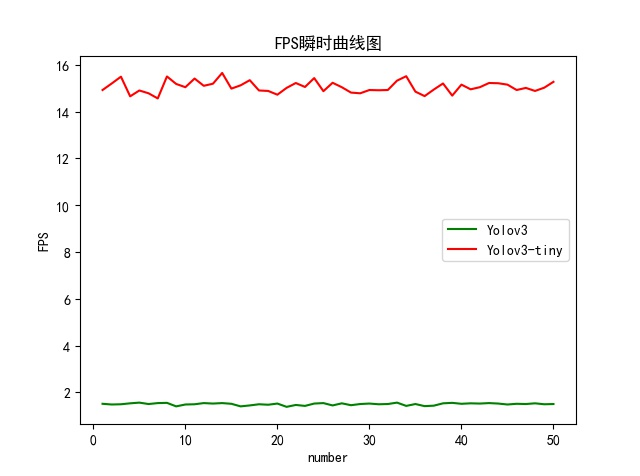
\includegraphics[width=0.46\columnwidth]{pic/chap5/FPS_plot.jpeg}
    }
    \subfigure[平均FPS柱状图]{
        \label{fig:FPS:average}
        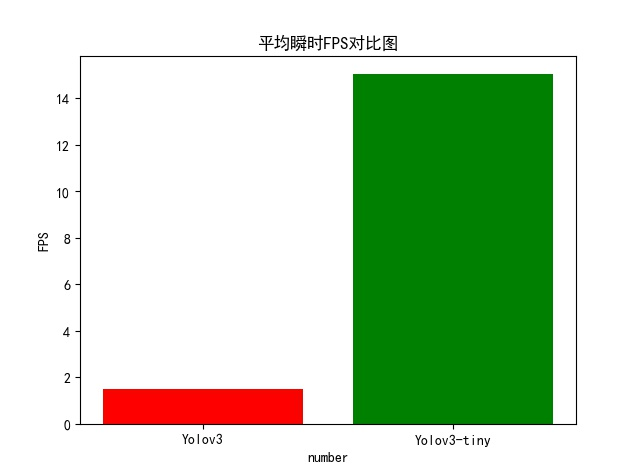
\includegraphics[width=0.46\columnwidth]{pic/chap5/average_FPS_plot.jpeg}
    }
    \caption{YOLOv3和YOLOv3-tiny部署后的FPS对比}
    \label{fig:FPS}
\end{figure}

由数据表及上图可知,YOLOv3部署后的FPS值稳定在1.50附近,平均值为1.4948;YOLOv3-tiny部署后的FPS值稳定在15.0附近,平均值为15.0536。
YOLOv3-tiny的FPS约为YOLOv3的10倍,即YOLOv3-tiny在一秒内能够处理的图片数量十倍于YOLOv3。

此外,实验还比较了两者在实验环境的新数据下的分类准确率。比较参数为51次实验情况下,每个工件的分类准确率。实验数据采集如下表:

{
    \begin{table}[htb] 
        \zihao{5}
        \caption{YOLOv3分类准确率实验数据采集表}
        \label{table:classification:YOLOv3_data}
        \centering
        \begin{tabular}[t]{c|c|c|c|c|c|c|c|c|c|c|c|c|c|c|c|c|c}
            \hline
            \diagbox{模型配置}{实验编号} & 1 & 2 & 3 & 4 & 5 & 6 & 7 & 8 & 9 & 10 & 11 & 12 & 13 & 14 & 15 & 16 & 17\\
            \hline
            dabai是否正确分类 & 1 & 1 & 0 & 1 & 1 & 1 & 1 & 1 & 1 & 1 & 1 & 1 & 1 & 1 & 1 & 1 & 1\\
            fo是否正确分类 & 1 & 1 & 1 & 1 & 1 & 1 & 1 & 1 & 1 & 1 & 1 & 1 & 1 & 1 & 1 & 0 & 1\\
            \hline
            & 18 & 19 & 20 & 21 & 22 & 23 & 24 & 25 & 26 & 27 & 28 & 29 & 30 & 31 & 32 & 33 & 34 \\
            \hline
            dabai是否正确分类 & 1 & 1 & 1 & 1 & 1 & 1 & 1 & 1 & 1 & 0 & 1 & 1 & 1 & 1 & 1 & 1 & 1\\
            fo是否正确分类 & 1 & 1 & 1 & 1 & 1 & 1 & 1 & 1 & 1 & 1 & 1 & 1 & 1 & 1 & 1 & 1 & 1\\
            \hline
            & 35 & 36 & 37 & 38 & 39 & 40 & 41 & 42 & 43 & 44 & 45 & 46 & 47 & 48 & 49 & 50 & 51\\
            \hline
            dabai是否正确分类 & 1 & 1 & 1 & 1 & 1 & 1 & 1 & 1 & 1 & 1 & 1 & 1 & 1 & 1 & 1 & 1 & 1\\
            fo是否正确分类 & 1 & 0 & 1 & 1 & 1 & 1 & 0 & 1 & 1 & 1 & 1 & 1 & 1 & 1 & 1 & 1 & 1\\
            \hline
        \end{tabular}
    \end{table}
}

{
    \begin{table}[htb] 
        \zihao{5}
        \caption{YOLOv3-tiny分类准确率实验数据采集表}
        \label{table:classification:YOLOv3-tiny_data}
        \centering
        \begin{tabular}[t]{c|c|c|c|c|c|c|c|c|c|c|c|c|c|c|c|c|c}
            \hline
            \diagbox{模型配置}{实验编号} & 1 & 2 & 3 & 4 & 5 & 6 & 7 & 8 & 9 & 10 & 11 & 12 & 13 & 14 & 15 & 16 & 17\\
            \hline
            dabai是否正确分类 & 1 & 1 & 0 & 1 & 1 & 1 & 1 & 1 & 1 & 1 & 1 & 1 & 1 & 1 & 0 & 1 & 1\\
            fo是否正确分类 & 1 & 1 & 1 & 1 & 1 & 1 & 1 & 0 & 1 & 1 & 1 & 1 & 1 & 1 & 1 & 1 & 1\\
            \hline
            & 18 & 19 & 20 & 21 & 22 & 23 & 24 & 25 & 26 & 27 & 28 & 29 & 30 & 31 & 32 & 33 & 34 \\
            \hline
            dabai是否正确分类 & 1 & 1 & 1 & 1 & 1 & 1 & 1 & 0 & 1 & 1 & 1 & 1 & 1 & 1 & 1 & 1 & 1\\
            fo是否正确分类 & 1 & 1 & 1 & 1 & 0 & 1 & 1 & 1 & 1 & 1 & 1 & 1 & 1 & 1 & 1 & 0 & 1\\
            \hline
            & 35 & 36 & 37 & 38 & 39 & 40 & 41 & 42 & 43 & 44 & 45 & 46 & 47 & 48 & 49 & 50 & 51\\
            \hline
            dabai是否正确分类 & 1 & 1 & 1 & 1 & 1 & 1 & 1 & 1 & 1 & 1 & 1 & 1 & 1 & 1 & 0 & 1 & 1\\
            fo是否正确分类 & 1 & 1 & 1 & 1 & 1 & 1 & 1 & 1 & 1 & 1 & 1 & 1 & 1 & 1 & 1 & 1 & 1\\
            \hline
        \end{tabular}
    \end{table}
}

表中,1代表正确分类,0代表没有正确分类。分类准确率的计算方式为:
\begin{equation}
    \centering
    \mbox{分类准确率}=\mbox{正确分类样本数}/\mbox{总样本数}
    \label{acc}
\end{equation}

两种模型配置的正确分类数量和分类准确率情况对比如图\ref{fig:classification:compare}所示。

由图可知,YOLOv3的分类准确率略高于YOLOv3-tiny,但两者相差不大,而YOLOv3-tiny部署在Jetson TX2后的图像处理性能十倍于YOLOv3,因此针对本自动分拣系统,
YOLOv3-tiny的模型配置具备相当的优越性,本文最终也选定YOLOv3-tiny作为最终部署在自动分拣系统当中的目标检测算法的模型配置。

\begin{figure}[h]
    \centering
    \subfigure[YOLOv3和YOLOv3-tiny分类情况]{
        \label{fig:classification:num}
        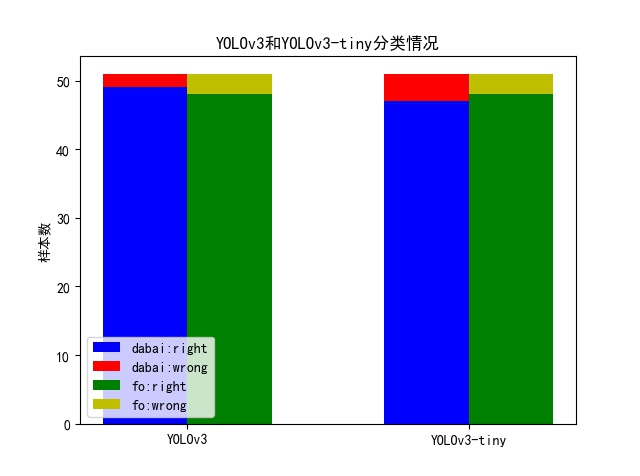
\includegraphics[width=0.46\columnwidth]{pic/chap5/classification_num.jpeg}
    }
    \subfigure[YOLOv3和YOLOv3-tiny分类准确率对比]{
        \label{fig:classification:acc}
        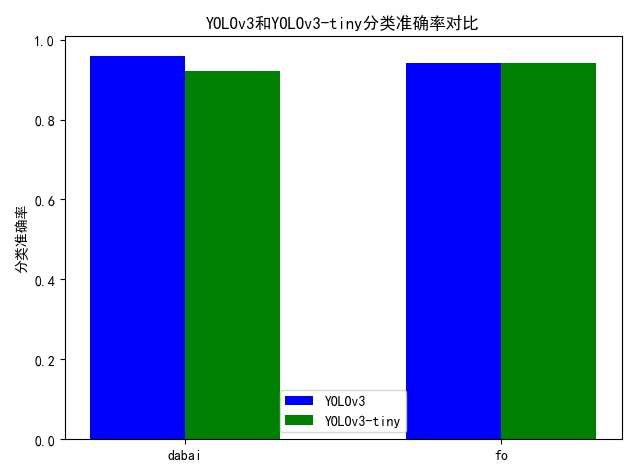
\includegraphics[width=0.46\columnwidth]{pic/chap5/classification_acc.jpeg}
    }
    \caption{YOLOv3和YOLOv3-tiny部署后的分类性能对比}
    \label{fig:classification:compare}
\end{figure}



\subsection{自动分拣系统分拣性能实验}

采用YOLOv3-tiny模型配置作为自动分拣系统图像处理模块的目标检测算法的配置进行部署,具体配置参数见表\ref{table:model:config}。
本小节将对自动分拣系统的分拣性能进行实验。分拣性能评估的是自动分拣系统能够成功抓取工件并将其正确分类的能力。因此,本实验将评估
两个实验数据:抓取成功率和分拣成功率。其中,分拣成功代表自动分拣系统将工件抓取到了正确的位置。即,抓取成功不代表分拣成功,而分拣成功代表一定抓取成功。
分拣成功率是更加严格的评估指标。抓取成功率代表自动分拣系统识别工件边框的准确能力,分拣成功率代表自动分拣系统的功能实现准确率。两者的计算方式如下:
$$\mbox{抓取成功率}=\mbox{机械臂成功抓取样本数}/\mbox{总样本数}$$
\begin{equation}
    \centering
    \mbox{分拣成功率}=\mbox{成功抓取到正确位置的样本数}/\mbox{总样本数}
    \label{fenjian}
\end{equation}

分别将两种工件dabai和fo放置在自动分拣系统的摄像头下,观测其抓取情况,记录其抓取成功和分拣成功的情况。
其中,工件dabai的数据记录表如表\ref{table:fenjian:dabai}所示;
工件fo的数据记录表如表\ref{table:fenjian:fo}所示。

{
    \begin{table}[htb] 
        \zihao{5}
        \caption{针对工件dabai的分拣性能实验数据记录表}
        \label{table:fenjian:dabai}
        \centering
        \begin{tabular}[t]{c|c|c|c|c|c|c|c|c|c|c|c|c|c|c|c|c|c}
            \hline
            \diagbox{参数}{实验编号} & 1 & 2 & 3 & 4 & 5 & 6 & 7 & 8 & 9 & 10 & 11 & 12 & 13 & 14 & 15 & 16 & 17\\
            \hline
            是否成功抓取 & 1 & 1 & 1 & 0 & 1 & 1 & 1 & 1 & 1 & 1 & 1 & 1 & 1 & 1 & 1 & 0 & 1\\
            是否正确分拣 & 1 & 1 & 1 & 0 & 1 & 1 & 1 & 1 & 1 & 1 & 1 & 1 & 1 & 1 & 0 & 0 & 1\\
            \hline
            & 18 & 19 & 20 & 21 & 22 & 23 & 24 & 25 & 26 & 27 & 28 & 29 & 30 & 31 & 32 & 33 & 34 \\
            \hline
            是否成功抓取 & 1 & 1 & 1 & 1 & 1 & 1 & 1 & 1 & 1 & 1 & 1 & 1 & 1 & 1 & 1 & 1 & 1\\
            是否正确分拣 & 1 & 1 & 1 & 1 & 1 & 1 & 1 & 1 & 1 & 1 & 1 & 1 & 1 & 1 & 1 & 1 & 1\\
            \hline
            & 35 & 36 & 37 & 38 & 39 & 40 & 41 & 42 & 43 & 44 & 45 & 46 & 47 & 48 & 49 & 50 & 51\\
            \hline
            是否成功抓取 & 1 & 1 & 1 & 1 & 1 & 1 & 1 & 1 & 1 & 1 & 1 & 1 & 1 & 1 & 1 & 1 & 1\\
            是否正确分拣 & 1 & 1 & 1 & 1 & 1 & 1 & 1 & 1 & 1 & 1 & 1 & 0 & 1 & 1 & 1 & 1 & 1\\
            \hline
        \end{tabular}
    \end{table}
}

{
    \begin{table}[htb] 
        \zihao{5}
        \caption{针对工件fo的分拣性能实验数据记录表}
        \label{table:fenjian:fo}
        \centering
        \begin{tabular}[t]{c|c|c|c|c|c|c|c|c|c|c|c|c|c|c|c|c|c}
            \hline
            \diagbox{参数}{实验编号} & 1 & 2 & 3 & 4 & 5 & 6 & 7 & 8 & 9 & 10 & 11 & 12 & 13 & 14 & 15 & 16 & 17\\
            \hline
            是否成功抓取 & 1 & 1 & 1 & 1 & 1 & 1 & 1 & 1 & 1 & 1 & 1 & 1 & 1 & 0 & 1 & 1 & 1\\
            是否正确分拣 & 1 & 1 & 1 & 1 & 1 & 1 & 1 & 1 & 1 & 1 & 1 & 0 & 1 & 0 & 1 & 1 & 1\\
            \hline
            & 18 & 19 & 20 & 21 & 22 & 23 & 24 & 25 & 26 & 27 & 28 & 29 & 30 & 31 & 32 & 33 & 34 \\
            \hline
            是否成功抓取 & 1 & 1 & 0 & 1 & 1 & 1 & 1 & 1 & 1 & 0 & 1 & 1 & 1 & 1 & 1 & 1 & 1\\
            是否正确分拣 & 1 & 0 & 0 & 1 & 1 & 1 & 1 & 1 & 1 & 0 & 1 & 1 & 1 & 1 & 1 & 1 & 1\\
            \hline
            & 35 & 36 & 37 & 38 & 39 & 40 & 41 & 42 & 43 & 44 & 45 & 46 & 47 & 48 & 49 & 50 & 51\\
            \hline
            是否成功抓取 & 1 & 1 & 1 & 1 & 1 & 1 & 1 & 1 & 1 & 1 & 1 & 1 & 1 & 1 & 1 & 1 & 1\\
            是否正确分拣 & 1 & 1 & 1 & 1 & 1 & 1 & 1 & 1 & 1 & 1 & 1 & 1 & 1 & 1 & 1 & 1 & 1\\
            \hline
        \end{tabular}
    \end{table}
}

两种工件的抓取成功率和分拣成功率计算如表\ref{table:fenjian:res}所示。由表可知,自动分拣系统的抓取成功率在95\%左右,
更为严格的分拣成功率则在91\%左右。基本达到可投入使用的水平。 

{
    \begin{table}[htb] 
        \zihao{5}
        \caption{分拣性能实验数据计算结果}
        \label{table:fenjian:res}
        \centering
        \begin{tabular}[t]{ccc}
            \hline
            工件 & 抓取成功率 & 分拣成功率\\
            \hline
            dabai & 96.08\% & 92.16\% \\
            fo & 94.12\% & 90.20\% \\
            \hline
        \end{tabular}
    \end{table}
}



\section{基于深度学习的目标检测模型云平台性能测试}
 
\subsection{Web前端性能测试实验}  
 
在基于深度学习的目标检测模型训练云平台中,
Web前端承担着与用户交互的任务,其性能表现好坏将直接影响用户使用的体验。本小节对Web前端页面的网络收发、页面渲染、js性能等进行测试,测试环境如表\ref{table:Web:env}所示。

{
    \begin{table}[htb]   
        \zihao{5}
        \caption{Web前端性能测试环境}
        \label{table:Web:env}
        \centering
        \begin{tabular}[t]{ccccc}
            \hline
            设备 & 操作系统 & CPU & 内存 & 浏览器\\
            \hline
            Macbook Pro 2018 & macOS & 8核 2.2GHZ & 16GB & safari \\
            \hline
        \end{tabular}
    \end{table}
}

将safari的开发选项调至菜单栏,使用其时间线录制工具,录制深度学习云平台Home界面的接收和渲染情况。
实验结果如图\ref{fig:web:test}所示。
由图可以看出,深度学习云平台的Web页面网络收发用时在xxms以内,页面渲染用时在xxms以内,js响应用时在xxms以内。收发数据量大小为xxB。可以看出,云平台的Web前端页面
的各项性能均非常优异。这种优异的性能主要来源于Bootstrap框架的优化和云平台页面本身的简洁性。

%%% TODO: safari时间线录制

而Web前端页面占用设备的资源情况如图\ref{fig:web:resource}所示。由图可以看出,深度学习云平台占用CPU情况,能耗情况均处于较低水平,不影响设备的正常使用。

%%% TODO: web页面占用资源图

\subsection{服务器端性能测试实验}

深度学习云平台的服务端服务于每个使用云平台的用户,其性能同样影响着用户体验。深度学习云平台所使用服务器配置如表\ref{table:server:config}。
测试用客户端参数如表\ref{table:Web:env}所示。本小节将对深度学习云平台服务端进行压力测试,
测试其承载能力。主要关注参数为能够同时承载的用户数量、服务器响应耗时等。

本实验使用Locust\cite{locust}为工具进行服务器压力测试实验。其参数设置如表\ref{table:locust:param}所示。在本次实验中,我们测试了5000个用户
同时使用云平台的情况。具体模拟情况为:用户数从0开始,每秒增加20个用户,每个用户的模拟行为为访问云平台主页一次和点击两次开始训练按钮,
每个用户的每次行为之间的间隔为5-15s之间的随机数。测试请求采用的通信协议为HTTP通信协议,访问云平台主页为GET请求方法,点击开始训练按钮为POST请求方法。
测试的链接即云平台网站域名:http://10.79.21.157:5000。
测试客户端与云平台服务器同处于校园局域网下,其IP地址为ZJUWLAN所分配的动态IP地址。

{
    \begin{table}[htb]   
        \zihao{5}
        \caption{Locust测试环境参数}
        \label{table:locust:param}
        \centering
        \begin{tabular}[t]{cccc}
            \hline
            用户数 & 每秒产生用户数 & 用户行为 & 用户行为间隔 \\
            \hline
            5000 & 20 & 访问主页1次+点击按钮2次  & random(5-15s) \\
            \hline
        \end{tabular}
    \end{table}
}

%%% TODO: Locust 图表分析,服务器性能分析(使用sar,记录实验期间期间服务器的情况)


\section{本章小结}

本章主要对本文设计的两部分系统:自动分拣系统和深度学习训练云平台进行了性能实验。第一节介绍了对自动分拣系统算法选择的
优越性进行了验证,然后验证了本文设计的基于深度学习目标检测算法的自动分拣系统的可用性与准确性。第二节介绍了本文设计开发的
深度学习云平台Web前端和服务器端的可用性与稳定性实验。

\chapter{总结与展望}

\section{总结}

分拣作业是制造业中非常常见的一种作业场景,由于其重复性强、作业场景单一的任务特性,分拣作业成为工业机器人的重要应用场景之一。传统的自动分拣
系统使用传统图像方法,针对特定的检测工件,人工构造特征,使用模板匹配工件位置,再进行分类。该方法准确率不高,鲁棒性差,可移植性不强。同时,国内
制造业从业者中缺乏图像方面的人才,提高了基于视觉的自动分拣系统在制造业中的应用门槛。因此,针对基于视觉的自动分拣系统的算法效果及其应用门槛问题,
研究如何提高自动分拣系统的应用效果并降低其在制造业中的应用门槛势在必行。

为了解决传统分拣系统所使用的传统目标检测算法存在的问题,本文设计的自动分拣系统采用基于深度学习的目标检测算法,并针对自动分拣系统的应用场景针对性地
进行了硬件选型、算法训练优化和模型配置文件优化,在提高了自动分拣系统算法效果的同时,又不降低其延时等性能。为解决制造业中,深度学习理论和应用普及度不广,
基于深度学习的自动分拣系统在制造业中应用门槛较高的问题,本文设计并开发了一款用于深度学习目标检测算法训练的云平台,将模型训练深度封装,并将模型配置过程
组件化,方便用户定制化深度学习目标检测模型。本文的主要工作内容如下:

(1) 设计自动分拣系统的整体架构,并针对性进行硬件、通信方式和基于深度学习的目标检测算法选型

结合基于视觉的自动分拣系统的原理,设计出应用层-控制层-云层的逻辑架构,将自动分拣系统的表现层面(抓取工件与获取图像)、控制层面(图像处理和机械臂控制)以及
后台层面(目标检测算法训练与选择)有机地分离开来,使得自动分拣系统的各模块呈现出松耦合的关系,方便后续深度学习云平台的开发;同时,结合自动分拣系统使用基于深度学习
的目标检测算法的情况,采用Jetson TX2作为中央处理单元,提供强大的算力以支持深度学习模型的预测,设计出工件-摄像头-Jetson TX2-DOBOT机械臂-工件的系统循环硬件架构。
此外,结合硬件系统架构,针对性地进行通信方式的选择,选择ROS作为Jetson TX2内部模块的通信机制,并使用ROS Mater节点将Jetson TX2内部各模块组织管理起来;结合
应用于工厂环境的自动分拣系统的实际情况,进行了深度学习目标检测算法的选型,选定YOLOv3作为应用于自动分拣系统的目标检测算法;最后,针对摄像头和机械臂,进行了手眼标定和
机械臂控制指令方案的设计与实现。

(2)设计自动分拣系统图像处理模块,结合传统图像算法和深度学习目标检测算法,使用迁移学习技术解决数据量较少的问题

本文设计的自动分拣系统采用基于深度学习的目标检测算法,相比于传统的目标检测算法,前者具有准确率高、鲁棒性强、可移植性强的优点。但深度学习模型需要大量的计算资源,
计算复杂度较高,因此本文在将图片输入深度学习模型中之前,首先使用传统图像算法进行初步处理,满足一定条件时才输入深度学习模型中,从而避免不必要的计算,提高运算速度。
此外,深度学习模型一般需要大量的数据作为训练样本,而工厂中很难有巨量的样本,更难靠人工标注的方式产生足够的样本。结合此实际情况,本文采用迁移学习技术,采用基于ImageNet
预训练的模型权重作为初始权重,结合小数量标注样本进行训练,从而获得更好的效果。在选择深度学习模型配置时,本文使用实验的方式,结合LOSS曲线和IOU曲线对YOLOv3和YOLOv3-tiny
两种模型配置进行了对比,最终得出针对本任务,YOLOv3-tiny更具优越性的结论。最后,训练好的模型还无法应用于实际场景,本文对训练好的深度学习模型进行了部署,将其加入到Jetson TX2的
ROS通信网络中,实现在自动分拣系统中进行目标检测的功能。

(3)设计并开发基于深度学习目标检测模型的云平台,降低深度学习目标检测模型的训练与使用门槛

结合云平台实际使用场景和用户需求,设计出Web-服务器的开发方案,并设计出客户端层-传输层-服务器层的云平台架构方案。本文主要完成了Web前端页面的开发和服务端驻留程序的开发。借助
Web前端页面的文本下拉选择框和文本输入框,用户可以通过简单的鼠标和键盘操作,即可配置相应的深度学习目标检测模型,通过自己上传的标注数据,训练定制化的深度学习目标检测模型。服务端
采用Flask架构,结合Linux Shell脚本,实现后台调用GPU训练用户定制化的目标检测模型。同时,在训练过程中,将训练参数实时反馈给用户,可由用户自主决定是否停止训练。在训练完成后,用户
可通过Web前端界面下载训练好的模型权重。该权重文件不单能够应用在自动分拣系统中进行工件检测,也可用于任何目标检测的任务场景。

本文设计开发的基于深度学习的自动分拣系统,在改进传统自动分拣系统目标检测算法不足并给出改进意见:采用基于深度学习的目标检测算法的同时,也基于此进行了硬件选型、模型训练
等方面的改进,同时提出的深度学习云平台大大降低了本系统在制造业中的应用门槛。


\section{展望}

本文主要对基于传统目标检测算法的自动分拣系统进行了改进,使用基于深度学习的目标检测算法替代了传统目标检测算法并进行了针对性改进,并开发出深度学习云平台用于降低该自动分拣系统的
应用门槛。但本文设计的基于深度学习的自动分拣系统及其云平台依然有进一步的研究与改进空间:

(1)硬件方面,采用Jetson TX2作为自动分拣系统的中央处理硬件平台,不仅提高了系统的运算能力,支持深度学习预测功能,并且大大缩小了自动分拣系统的体积,使得可移动的自动分拣系统成为可能。
因此,本系统具备进一步的研究空间,可将机械臂放置于运动载具上,进行移动式自动分拣系统的研究。

(2)本文在解决小数量标注数据集问题时,采用了模型迁移的迁移学习方式,即采用预训练模型权重作为本任务模型的初始化权重进行训练。该方式经过验证确实提高了采用小数量数据训练模型的表现,但
在模型迁移之外,还可以探索数据迁移等迁移学习方式,尽可能地提高小数量数据集训练模型的表现。

(3)为降低深度学习自动分拣系统的应用门槛,本文开发了用于训练深度学习目标检测模型的云平台。该平台依然有大量的优化空间。如增加模型封装范围,云平台将模型训练过程进行了封装,而模型部署
依然需要用户进行。因此可以考虑将模型训练、模型部署过程一起封装,用户只需关注自动分拣系统硬件的组装,软件模块可一件脚本执行部署完成。此外,因为该平台是针对本文设计的自动分拣系统所设计,因此
平台只支持深度学习目标检测算法的训练。而制造业中有许多图像算法的应用场景,如图像分类、图像分割等,可考虑增加可训练的模型种类,扩大云平台应用范围。
 
\ZJUbackmatter
%%%%%%%%%%%%%%%%%%%%%%%%%%%%%%
%% 参考文献
%%%%%%%%%%%%%%%%%%%%%%%%%%%%%%
\ZJUthesisbib{thesisbib}

%%%%%%%%%%%%%%%%%%%%%%%%%%%%%%
%% 附录
%%%%%%%%%%%%%%%%%%%%%%%%%%%%%%
%\appendix
%\chapter{附录A}

这是附录A的内容。

\chapter{附录B}

这是附录B的内容。



%%%%%%%%%%%%%%%%%%%%%%%%%%%%%%
%% 索引
%%%%%%%%%%%%%%%%%%%%%%%%%%%%%%
%\ZJUindex

\end{document}
 